% ---------------------------------------------------------------------------
% IEEE ICDE 2027, Research Track (Data Security and Privacy).
% IEEE conference format: at most 12 pages, excluding references and the
% AI-generated content acknowledgement; no appendix. Single-blind review.
%   tectonic --keep-logs --keep-intermediates main.tex
%
% Active numerical objects are generated from immutable experimental records:
%   python experiments/release-value-20261019/src/export_value.py --paper paper
% Run from the packaged project root; do not edit numerical table cells.
% ---------------------------------------------------------------------------
\documentclass[conference]{IEEEtran}

\usepackage{iftex}
\ifXeTeX\usepackage{fontspec}\setmainfont{texgyretermes}[Extension=.otf,UprightFont=*-regular,BoldFont=*-bold,ItalicFont=*-italic,BoldItalicFont=*-bolditalic]\setmonofont{texgyrecursor}[Extension=.otf,UprightFont=*-regular,BoldFont=*-bold,ItalicFont=*-italic,BoldItalicFont=*-bolditalic]\fi
\usepackage{booktabs}
\usepackage{array}
\usepackage{etoolbox}
% IEEE tables use footnotesize; generated table files request \small.
\AtBeginEnvironment{table}{\let\small\footnotesize}
\AtBeginEnvironment{table*}{\let\small\footnotesize}
\usepackage{graphicx}
\usepackage{tikz}
\usetikzlibrary{arrows.meta,positioning,fit,decorations.pathreplacing}
\usepackage{enumitem}
\usepackage{algorithm}
\usepackage{algpseudocode}
\usepackage{amsmath,amssymb,amsfonts}
\usepackage{amsthm}
\usepackage{cite}
\usepackage[hidelinks]{hyperref}
\newtheorem{lemma}{Lemma}
\newtheorem{theorem}{Theorem}
\newtheorem{valueprop}{Proposition}
\theoremstyle{definition}
\newtheorem{definition}{Definition}
\providecommand{\Description}[1]{}
\setlength{\emergencystretch}{2em}

% Generated numerical prose values.
\newcommand{\FixedGlobal}{90.7\%}
\newcommand{\FixedGlobalSd}{4.2\%}
\newcommand{\FixedClient}{85.7\%}
\newcommand{\MixHalf}{85.0\%}
\newcommand{\MixFull}{89.8\%}
\newcommand{\MixNN}{89.7\%}
\newcommand{\MixGain}{4.8}
\newcommand{\MixGainCI}{[3.5,6.0]}
\newcommand{\MixFinal}{88.5\%}
\newcommand{\CifChosenGlobal}{91.6\%}
\newcommand{\CifChosenClient}{86.3\%}
\newcommand{\CifHead}{92.4\%}
\newcommand{\CifCTClient}{71.3\%}
\newcommand{\CifStudent}{91.9\%}
\newcommand{\CifCTStudent}{87.5\%}
\newcommand{\WebChosenGlobal}{24.8\%}
\newcommand{\WebChosenClient}{25.5\%}
\newcommand{\WebCTClient}{21.8\%}
\newcommand{\WebGain}{3.7}
\newcommand{\WebGainCI}{[2.0,5.5]}
\newcommand{\FemLowGlobal}{17.3\%}
\newcommand{\FemLowClient}{31.5\%}
\newcommand{\FemLocal}{32.2\%}
\newcommand{\FemLowMacro}{10.8\%}
\newcommand{\FemLocalMacro}{11.9\%}
\newcommand{\FemHighGlobal}{30.2\%}
\newcommand{\FemHighClient}{32.5\%}
\newcommand{\FemHighMacro}{10.3\%}
\newcommand{\FemPublicMatched}{50.6\%}
\newcommand{\FemPublicSelected}{59.3\%}
\newcommand{\FemLocalPublic}{37.6\%}
\newcommand{\QuerySemantic}{82.9\%}
\newcommand{\QueryUniform}{58.9\%}
\newcommand{\QueryGain}{24.0}
\newcommand{\QueryGainCI}{[21.5,26.5]}

% Generated from all retained label draws and paired cohorts.
\newcommand{\BudgetGain}{6.6}
\newcommand{\BudgetGainCI}{[0.9,12.4]}
\newcommand{\RandomPublicTen}{59.7\%}
\newcommand{\RandomHybridTen}{66.3\%}
\newcommand{\RandomPortfolioTen}{55.7\%}
\newcommand{\CifSingle}{91.6\%}
\newcommand{\CifHeadSingle}{93.9\%}
\newcommand{\CifRoundGain}{2.3}
\newcommand{\CifSmallSingle}{52.2\%}
\newcommand{\CifSmallHeadSingle}{32.8\%}
\newcommand{\CifSmallRoundGain}{12.2}
\newcommand{\FemLowSingle}{19.8\%}
\newcommand{\FemLowHeadSingle}{26.3\%}
\newcommand{\FemLowRoundGain}{10.6}
\newcommand{\FemHighSingle}{35.6\%}
\newcommand{\FemHighHeadSingle}{41.3\%}
\newcommand{\FemHighRoundGain}{3.6}

% Generated: independent joint-naming confirmation.
\newcommand{\JointGain}{13.0}
\newcommand{\JointGainCI}{[4.6,21.4]}
\newcommand{\JointPublic}{61.6\%}
\newcommand{\JointAccuracy}{74.6\%}
\newcommand{\JointPortfolio}{56.1\%}

% Generated analysis and private verification results.
\newcommand{\GainMedian}{13.6}
\newcommand{\GainFifth}{-3.8}
\newcommand{\GainNegativeDraws}{9}
\newcommand{\GainNegativeCases}{16}
\newcommand{\LabelAxisSD}{10.11}
\newcommand{\CohortAxisSD}{7.95}
\newcommand{\TightGlobalAccept}{4.6}
\newcommand{\TightClassAccept}{0.0}
\newcommand{\MiddleGlobalAccept}{86.8}
\newcommand{\MiddleClassAccept}{6.2}
\newcommand{\LargerGlobalAccept}{87.0}
\newcommand{\LargerClassAccept}{75.9}

% Generated: EAB revision analyses (export_eab.py).
\newcommand{\CeilCifar}{91.6}
\newcommand{\CeilMnist}{52.6}
\newcommand{\CeilUsenet}{42.4}
\newcommand{\CeilFemnistOne}{24.6}
\newcommand{\CeilFemnistMany}{42.9}
\newcommand{\RoomCifar}{30.0}
\newcommand{\RoomMnist}{6.4}
\newcommand{\RoomUsenet}{10.3}
\newcommand{\RoomFemnist}{-12.7}
\newcommand{\NamedMnist}{52.6}
\newcommand{\NamedUsenet}{20.7}
\newcommand{\NamedCifarOne}{50.3}
\newcommand{\NoiseCifarOne}{0.215}
\newcommand{\NoiseCifarTen}{0.022}
\newcommand{\NoiseUsenet}{0.006}
\newcommand{\JointMnist}{44.4}
\newcommand{\HeadMnist}{72.2}
\newcommand{\PublicMnist}{46.2}
\newcommand{\LadderGainTwoTenth}{58.2}
\newcommand{\LadderRecallHalfThree}{0.0}
\newcommand{\LadderRecallQuarterThree}{75.7}
\newcommand{\LadderNondegHalf}{83.1}
\newcommand{\LadderNondegQuarter}{2.0}
\newcommand{\AllocClassOneRef}{65.2}
\newcommand{\AllocClassOneSel}{88.5}
\newcommand{\AllocClassOneGain}{23.3}
\newcommand{\AllocClassOneCI}{[22.62,23.90]}
\newcommand{\AllocHalfThreeRef}{62.8}
\newcommand{\AllocHalfThreeSel}{85.0}
\newcommand{\AllocGainTenth}{1.7}
\newcommand{\AllocGainTenthCI}{[-0.04,3.47]}
\newcommand{\AllocGainThird}{2.4}
\newcommand{\AllocGainThirdCI}{[-0.32,5.21]}

% Generated: third EAB round (export_eab3.py).
\newcommand{\CleanUsenet}{32.3}
\newcommand{\CleanMnist}{53.9}
\newcommand{\CleanFemnist}{35.3}
\newcommand{\TeacherFemnist}{7.5}
\newcommand{\NoiseLossFemnistTenth}{15.5}
\newcommand{\NoiseLossFemnistOneTenth}{28.3}
\newcommand{\RoomFemnistMany}{5.5}
\newcommand{\NoiseLossCifarOne}{41.2}
\newcommand{\NoiseLossUsenet}{11.6}
\newcommand{\SelLossMnist}{8.2}
\newcommand{\NamedCifarTen}{91.6}
\newcommand{\SelLossCifarTen}{4.2}
\newcommand{\GateVzero}{0.03}
\newcommand{\GatedMnistHeld}{+7.3}
\newcommand{\LooMnistHeld}{-2.2}
\newcommand{\GatedCifarTenHeld}{+27.7}
\newcommand{\LooCifarTenHeld}{+24.2}
\newcommand{\GatedUsenetHeld}{-11.3}
\newcommand{\LooUsenetHeld}{-4.0}
\newcommand{\GatedMnistGain}{+6.4}
\newcommand{\GatedMnistCI}{[4.7,8.0]}
\newcommand{\CoverCifarOne}{-11.3}
\newcommand{\AuditCifarOneEst}{92.5}
\newcommand{\AuditCifarOneHeld}{62.2}
\newcommand{\AuditCifarFiveEst}{91.6}
\newcommand{\AuditCifarFiveHeld}{91.6}
\newcommand{\AuditMnistTwentyEst}{55.5}
\newcommand{\AuditMnistTwentyHeld}{51.0}
\newcommand{\AuditMnistFiftyEst}{54.9}
\newcommand{\AuditMnistFiftyHeld}{51.5}
\newcommand{\AuditUsenetFiftyEst}{45.8}
\newcommand{\AuditUsenetFiftyHeld}{40.2}
\newcommand{\AuditUsenetTrue}{42.4}
\newcommand{\AuditFemnistTwentyEst}{26.4}
\newcommand{\AuditFemnistTwentyHeld}{20.7}
\newcommand{\AuditFemnistTrue}{24.6}
\newcommand{\GatedUsenetLoss}{7.3}
\newcommand{\MinRecGainOnePub}{868}
\newcommand{\MinRecGainOneZero}{6.6}
\newcommand{\MinRecGainOneTenth}{12.7}
\newcommand{\MinRecGainThreeTenth}{12.8}
\newcommand{\MinRecClassThreeMedian}{85.0}
\newcommand{\MinRecClassThreeLow}{85.0}
\newcommand{\PlanMaxGap}{1.1}
\newcommand{\PlanCells}{18}
\newcommand{\PlanGain}{27.5}
\newcommand{\PlanMinRecall}{81.8}
\newcommand{\PlanMinDiff}{0.0}
\newcommand{\PlanAnchorGainTenth}{0.3}
\newcommand{\PlanAnchorRecallZero}{1.3}
\newcommand{\PlanAnchorRecallQuarter}{2.3}
\newcommand{\PlanAnchorRecallHalf}{5.1}
\newcommand{\PlanAnchorNondegHalf}{2.5}
\newcommand{\PlanAnchorNondegQuarter}{4.4}
\newcommand{\PlanRecallZeroCSixtyTwo}{11.6}
\newcommand{\PlanRecallZeroNTenK}{0.13}

% Generated: gated rule + private verification confirmation (export_eab4.py).
\newcommand{\VTCases}{6000}
\newcommand{\VTMnistAccept}{99.6}
\newcommand{\VTUsenetAccept}{20.6}
\newcommand{\VTCifarAccept}{98.0}
\newcommand{\VTUsenetPriv}{495}
\newcommand{\VTUsenetAccepted}{102}
\newcommand{\VTMnistGatedLoo}{+10.6}
\newcommand{\VTUsenetGatedLoo}{-4.4}
\newcommand{\VTUsenetGatedLooCI}{[-8.3,-0.7]}
\newcommand{\VTMnistVerLoo}{+10.6}
\newcommand{\VTMnistVerLooCI}{[+8.0,+13.6]}
\newcommand{\VTUsenetVerLoo}{+0.5}
\newcommand{\VTUsenetVerLooCI}{[-0.7,+1.7]}
\newcommand{\VTUsenetAccAcc}{+15.8}
\newcommand{\VTUsenetAccBal}{+2.1}
\newcommand{\VTUsenetAccBalShare}{62.7}
\newcommand{\VTUsenetAccClean}{+0.155}
\newcommand{\VTUsenetRejAcc}{-15.1}
\newcommand{\VTUsenetRejBal}{-6.2}
\newcommand{\VTUsenetRejClean}{-0.139}
\newcommand{\VTUsenetRadius}{0.043}
\newcommand{\VTFalseAccepts}{0}
\newcommand{\VTMnistClassAccept}{0.0}
\newcommand{\VTSeeds}{10}
\newcommand{\VTFrozen}{2026-10-20}

% Generated: fifth EAB round (export_eab5.py).
\newcommand{\CeilMnistMany}{54.1}
\newcommand{\RoomMnistMany}{7.9}
\newcommand{\RoomCifarMany}{30.0}
\newcommand{\RoomUsenetMany}{10.3}
\newcommand{\TeachMnist}{+0.2}
\newcommand{\NoiseMnist}{+1.3}
\newcommand{\SelMnist}{+8.2}
\newcommand{\TeachUsenet}{10.2}
\newcommand{\SelCifarOne}{-24.3}
\newcommand{\NoiseImprMnist}{2/10}
\newcommand{\NoiseImprFemnist}{6/10}
\newcommand{\NoiseFemnistOne}{-0.2}
\newcommand{\BalUsenetAccept}{0.0}
\newcommand{\BalMnistAccept}{77.4}
\newcommand{\BalUsenetUtil}{28.2}
\newcommand{\BalMnistUtil}{52.3}
\newcommand{\AccMnistUtil}{53.6}
\newcommand{\UsenetAccVerAcc}{40.0}
\newcommand{\UsenetAccPubAcc}{36.7}
\newcommand{\TightRecallOne}{18.3}
\newcommand{\FixedRecallOne}{6.2}
\newcommand{\DisjGainImpr}{26.6}
\newcommand{\DisjGainCI}{[23.7,29.5]}
\newcommand{\ReusedGainImpr}{26.6}
\newcommand{\DisjGainAccOne}{86.7}
\newcommand{\DisjRecallThree}{77.1}
\newcommand{\DisjFAThree}{2}
\newcommand{\DisjMaxDiff}{1.4}
\newcommand{\DisjRecords}{32}
\newcommand{\DisjHeld}{8}
\newcommand{\DisjSources}{40000}
\newcommand{\PlanOOSGap}{0.5}
\newcommand{\PlanOOSCells}{12}
\newcommand{\UsenetMassMin}{0.055}
\newcommand{\UsenetMassMax}{0.387}
\newcommand{\MnistClassOne}{0.0}

% Generated: sixth EAB round (export_eab6.py).
\newcommand{\CalcCells}{24}
\newcommand{\CalcGap}{1.1}
\newcommand{\CostFixedRecallOne}{6.4}
\newcommand{\CostTightRecallOne}{19.8}
\newcommand{\CostRefRecallOne}{7.8}
\newcommand{\CostOptRecallOne}{81.8}
\newcommand{\CostOptRecallOneUtil}{88.5}
\newcommand{\CostRefRecallOneUtil}{65.2}
\newcommand{\CostOptRecallOnePhi}{.1}
\newcommand{\CostOptHalfThree}{70.2}
\newcommand{\HetDisjoint}{0.672}
\newcommand{\HetLast}{0.667}
\newcommand{\HetReused}{0.664}
\newcommand{\HetFree}{0.664}

% Generated: eighth EAB round (export_eab8.py).
\newcommand{\BCCases}{54000}
\newcommand{\BCCohorts}{10}
\newcommand{\BCRecTrain}{16}
\newcommand{\BCRecHeld}{4}
\newcommand{\BCPhiRecallOne}{.2}
\newcommand{\BCFixedRecallOne}{5.4}
\newcommand{\BCFrozenRecallOne}{78.2}
\newcommand{\BCFixedRecallOneUtil}{64.5}
\newcommand{\BCFrozenRecallOneUtil}{87.2}
\newcommand{\BCDiffRecallOneUtil}{+22.8}
\newcommand{\BCDiffRecallOneUtilCI}{[+18.9, +26.7]}
\newcommand{\BCDiffRecallOneAcc}{+72.8}
\newcommand{\BCDiffRecallOneAccCI}{[+62.0, +83.0]}
\newcommand{\BCPhiHalfThree}{.1}
\newcommand{\BCFrozenHalfThree}{76.2}
\newcommand{\BCFrozenHalfThreeUtil}{87.2}
\newcommand{\BCFixedHalfThreeUtil}{62.8}
\newcommand{\BCDevRecallOne}{69.4}
\newcommand{\BCFalseAccepts}{0}
\newcommand{\BCGainMaxDiff}{0.1}
\newcommand{\BCMaxRegret}{1.5}
\newcommand{\BCPilotRecallOne}{86.2}
\newcommand{\BCPilotHalfThree}{84.2}
\newcommand{\BCPilotSubsamples}{50}
\newcommand{\BCPoolImages}{22500}
\newcommand{\PointRegionMaxGap}{2.3}
\newcommand{\PointRegionSettings}{8}
\newcommand{\HeadMnistTenK}{72.2}
\newcommand{\RegionMnistTenK}{44.4}

\newcommand{\TauCerts}{47355}
\newcommand{\TauMaxLog}{-6.6\times10^{6}}
\newcommand{\ExtSeeds}{5}
\newcommand{\ExtSDDCifar}{85.0}
\newcommand{\ExtFedCTCifar}{69.7}
\newcommand{\ExtPATECifar}{80.5}
\newcommand{\ExtHeadCifar}{92.7}
\newcommand{\ExtSDDMnist}{55.0}
\newcommand{\ExtFedCTMnist}{46.2}
\newcommand{\ExtPATEMnist}{52.0}
\newcommand{\ExtHeadMnist}{67.3}
\newcommand{\EncCeilOne}{61.9}
\newcommand{\EncCeilMany}{62.2}
\newcommand{\EncPublic}{42.6}
\newcommand{\EncJoint}{38.6}
\newcommand{\EncGain}{$-$4.0}
\newcommand{\EncGainCI}{[$-$5.4,$-$2.6]}
\newcommand{\EncDirected}{61.9}
\newcommand{\EncHead}{28.1}
\newcommand{\EncPrivRate}{24}
\newcommand{\FCCases}{27000}
\newcommand{\FCPlanGap}{0.7}
\newcommand{\FCGainOne}{99.0}
\newcommand{\FCGainOneTrue}{100.0}
\newcommand{\FCClassMax}{0.0}
\newcommand{\FCTail}{100.0}
\newcommand{\FCFA}{0}
\newcommand{\FCUtilFixed}{35.1}
\newcommand{\FCPub}{11.6}

\newcommand{\PilotDevLabels}{100}
\newcommand{\PilotValLabels}{3967}
\newcommand{\PilotConfigs}{17}
\newcommand{\PilotReleases}{267}
\newcommand{\PilotRhoMult}{97.1}
\newcommand{\PilotEpsOne}{11.7}
\newcommand{\FCPublicPortfolio}{36.3}
\newcommand{\FCPublicBest}{37.2}
\newcommand{\MinNoiseScale}{1241}


\begin{document}

\title{[Experiment, Analysis, and Benchmark]\\ Private Supervision under
Strong Public Representations: Label Access, Release Granularity, and
Verification}

\author{\IEEEauthorblockN{Author Name(s)}
\IEEEauthorblockA{Affiliation\\
Email}}

\maketitle

\begin{abstract}
Strong public representations make task supervision the scarce resource
of a data-platform classifier: public labels under some acquisition
contract, or private client opinions reachable only through aggregate-only,
differentially private interfaces. This experiment and analysis paper
measures what private supervision adds and what verification costs, fixing
annotation budget and acquisition mode, whole-client privacy budget, report
payload, representation and public post-processing on four tasks; image
clients are simulated privacy units built from public benchmarks, Usenet
authors and FEMNIST writers are natural. Three findings stand out. First,
acquisition rights decide whether private reports are needed: with ten random
CIFAR labels at $\varepsilon=.1$, private regional naming adds \JointGain{}
points over the strongest of fourteen public learners, yet ten
feature-directed labels reach the same \CeilCifar{}\% classifier without
private reports. Second, raw sensitivity does not rank release interfaces:
per-example votes are about 14 times more sensitive than regional reports, but
pooled within regions they carry .88--1.07 times the regional noise and match
regional accuracy within \PointRegionMaxGap{} points; payload is what differs.
Third, publication evidence is a separate resource:
\MinRecGainOneTenth{}\% of the classifiers a mean-gain certificate publishes
recall some class below 10\%, and a budget split selected on independent
development cohorts and frozen raises all-class acceptance on new cohorts from
\BCFixedRecallOne{}\% to \BCFrozenRecallOne{}\% at $\varepsilon=1$, with no
false accept. The public artifact (\url{https://github.com/Xinbw/SDD})
regenerates every reported number.
\end{abstract}

\begin{IEEEkeywords}
differential privacy, experimental analysis, federated data, distributed DP,
data acquisition, public representations, private verification
\end{IEEEkeywords}

\section{Introduction}
\label{sec:intro}

Strong public representations have changed where the cost of a classifier
lies. A frozen vision or text encoder already places semantically similar
records near each other, so a data platform can expose class structure
before it owns a single task label. What remains scarce is
\emph{supervision}: public annotation, at a cost and under acquisition rights
that determine which examples may be requested, or private clients, such as
devices, organizations or user accounts, whose labelled records are reachable
only through protected aggregate interfaces.

A platform that wants to publish a classifier therefore makes three decisions
(Figure~\ref{fig:scenario}): \emph{what supervision to buy}, public labels or
private reports; \emph{what statistic to release} from clients, per-example
votes, a compact regional summary or a clipped model head; and \emph{what
evidence to require} before publication. Evaluated separately and judged by average
accuracy, reported gains mix these resources and do not transfer.

% Schematic (no data): the platform's three decisions (vector figure, experiments/release-eab9-20261021/figure-source).
\begin{figure}[t]
\centering
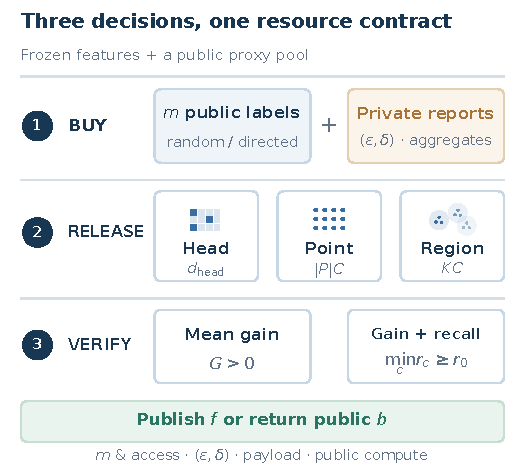
\includegraphics[width=.92\columnwidth,trim=0 .02in 0 .56in,clip]{figures/fig-decision-map.pdf}
\Description{Three platform decisions: buy public labels and/or private
reports, choose a release object (head, point or region), and choose the
verification target before publishing a candidate or the public comparator.}
\caption{Three platform decisions under a shared resource contract: the
acquisition contract for public labels and private supervision, the
protected release object, and the evidence required before publication.}
\label{fig:scenario}
\end{figure}


\subsection{An experiment and analysis study}

This paper is an experimental analysis, not a new release mechanism:
regional naming, distributed discrete-Gaussian aggregation and noisy-count
confidence bounds are established components. Its contribution is a
\emph{resource-matched evaluation protocol} and what it reveals. The
protocol measures private value against the strongest public learner with the
same labels, representation and acquisition mode (Section~\ref{sec:problem});
every comparison fixes annotation budget and acquisition mode, total
whole-client privacy budget, released coordinates and public post-processing,
and verification is charged to the same total budget as naming. We apply it
to 3426 inherited primary records over 90 cohorts and 4224 public label sets,
and to five studies whose designs were frozen before they ran
(Table~\ref{tab:studies}). Image clients are simulated privacy units built
from public benchmarks; Usenet authors and FEMNIST writers are natural.

\subsection{Findings}

\paragraph{Finding 1: acquisition rights decide private value}
With ten random CIFAR-1k labels at $(\varepsilon,\delta)=(.1,10^{-5})$, joint
naming beats the strongest of fourteen equal-budget public learners by
\JointGain{} points on average (median \GainMedian{}), though
\GainNegativeDraws{}\% of label draws lose. Ten feature-directed labels
recover the same \CeilCifar{}\% classifier without private reports: an
evaluation must fix both how many labels exist and how they are acquired.
With a weaker ResNet-18 encoder, directed labels again reach the partition
ceiling without private reports, but random-label joint naming changes the
strongest public learner by \EncGain{} points: passive private value also
needs regions that carry the classes.

\paragraph{Finding 2: raw sensitivity does not rank release interfaces}
Per-example votes on $|P|=2000$ proxy points are $\sqrt{|P|/K}\approx14$
times more sensitive than a $K=10$ regional report and need 20000 rather than
100 coordinates. Yet averaging point votes inside each region brings their
noise to .88--1.07 times the regional level, and pooled point and regional
joint naming differ by at most \PointRegionMaxGap{} points on all
\PointRegionSettings{} tested settings. The protected head, a different
object, wins where the partition limits regional naming (MNIST:
\HeadMnistTenK{} versus \RegionMnistTenK{}\%). Payload and partition fit, not
sensitivity, should choose the interface.

\paragraph{Finding 3: publication evidence is a separate resource}
On held-out clients charged to one total budget, a mean-gain certificate is
cheap, accepting \MiddleGlobalAccept{}\% of cases at $\varepsilon=1$, but
\MinRecGainOneTenth{}\% of the classifiers it publishes recall some test class
below $10\%$. Class evidence costs more, at a price set by the protocol. A naming share selected on independent
development cohorts, frozen, and confirmed on new cohorts and the test split
raises all-class acceptance from \BCFixedRecallOne{}\% to
\BCFrozenRecallOne{}\% at $\varepsilon=1$ ($\BCDiffRecallOneUtil$ test
accuracy points), makes recall $\ge.5$ certifiable at $\varepsilon=3$
(\BCFrozenHalfThree{}\%), leaves mean-gain release unchanged and records no
false accept. On natural FEMNIST writers, where no class target is reachable,
a calculator prediction frozen before confirmation lands within \FCPlanGap{}
points in every cell, and \FCTail{}\% of the classifiers the mean-gain rule
publishes recall some class below 10\%.

\paragraph{Explaining the losses}
Stored noise-free votes split the gap below the partition ceiling into signed
differences: teacher content dominates on Usenet, release noise on CIFAR-1k
and FEMNIST at $\varepsilon=.1$, selection on MNIST and CIFAR-10k. Private
verification of a noise-gated rule screens cases, not tasks.

\subsection{Contributions}
\begin{itemize}[leftmargin=*,itemsep=1pt,topsep=2pt]
\item A resource-matched evaluation protocol with annotation access, privacy
budget, payload and publication target as separate resources
(Section~\ref{sec:problem}), and a map of which information supports
deployment decisions (Section~\ref{sec:discussion}).
\item Three findings on what to buy, release and verify, with a weaker-encoder
ablation, published per-example and head baselines on the same protected sum,
a cost ladder, tighter-band and source-disjoint controls, a budget split
selected on independent cohorts and confirmed on CIFAR, and a
Gaussian-approximation acceptance calculator tested on natural FEMNIST writers
(Sections~\ref{sec:eval:main}--\ref{sec:eval:verification}).
\item Signed differences below a decoder-matched partition ceiling that
locate the loss on four tasks, and a pre-registered study of gated selection
plus verification (Section~\ref{sec:eval:ceiling}).
\item A public artifact that regenerates every number from immutable records
and replays protected outputs from retrained cohorts.
\end{itemize}

\section{Problem Formulation}
\label{sec:problem}

\subsection{Data roles}

A coordinator holds a public encoder $g$, an unlabelled \emph{proxy pool}
$P$ on which regions are formed, a \emph{development pool} whose labels are
revealed only under a declared acquisition mode, and a \emph{test pool}
used only offline. The class count and taxonomy are public; class
frequencies and external validation labels are not free.

Private data are held by $n$ clients. Client $i$ holds a labelled dataset
$D_i$ and may train a local model $f_i$; the coordinator observes clients
only through a protected sum over all participants, and the unit of
protection is a complete client dataset. For private verification, each
client also holds held-out records used only for bounded validation reports.

\subsection{Resources}

Each configuration carries a resource vector. \emph{Annotation}: $m$
distinct development labels and an acquisition mode, either \emph{random}
(uniform draws), \emph{balanced} ($m/C$ per class) or
\emph{feature-directed} (examples nearest each public region, requested
before any label is revealed); every fitting, selection and public
publication decision uses labels within $m$. \emph{Privacy}: one total
$(\varepsilon,\delta)$ budget under replace-one whole-client adjacency,
composed over all releases of a deployment. \emph{Payload}: integer
coordinates per client and release, before secret sharing.
\emph{Public computation}: decoding, assignment, selection and an optional
public student. Configurations differing in more than one resource are
reported as separate conditions.

\subsection{Release objects and endpoints}

A release object is the protected vector a client contributes: a clipped
parameter update, per-example proxy votes, or one bounded opinion per public
region. The published endpoint is a \emph{public classifier}; client models
are never published.

\subsection{Marginal value of private supervision}

Let $\mathcal H_{\mathrm{pub}}$ be a fixed family of public learners, each of
which maps a label set $L_m$ and the public features to a classifier. The
encoder is part of the resource vector: a zero-shot head on another
encoder, or one supervised by class names, changes the representation, not
$m$, and is compared as a separate condition. Let
$U(h)$ denote test accuracy (balanced accuracy for Usenet).

\begin{definition}[Resource-matched marginal value]
\label{def:value}
For acquisition mode $a$, budget $m$ and total privacy budget $\varepsilon$,
\begin{equation}
V_a(m,\varepsilon)=\mathbb E\bigl[U(h_{\mathrm{joint}})\bigr]
-\max_{h\in\mathcal H_{\mathrm{pub}}}\mathbb E\bigl[U(h)\bigr],
\label{eq:marginal-value}
\end{equation}
where $h_{\mathrm{joint}}$ combines the same label set with one protected
release under budget $\varepsilon$, and expectations run over label draws
from mode $a$ and over cohort/noise seeds.
\end{definition}

No within-budget selection rule is guaranteed to reach the maximum over
learner \emph{means}, so Eq.~\eqref{eq:marginal-value} is conservative. It
depends on $a$ as well as $m$, and since a deployment sees one label draw and
one cohort, we also report the per-draw gain distribution.

\subsection{Publication targets}

A positive $V_a$ concerns average utility; a publishing coordinator may
require more. We consider two targets for a candidate $f$ against a fixed public comparator $b$. The \emph{gain target}
requires the finite held-out cohort mean $G=n^{-1}\sum_i
[u_i(f)-u_i(b)]$ to be positive, where $u_i$ is held-out accuracy at client
$i$. The \emph{classwise target} additionally requires every client-weighted
class recall $\sum_i \mathrm{TP}_{i,c}/H_i\,/\sum_i N_{i,c}/H_i$ to be positive
($H_i$ held-out records at client $i$, $N_{i,c}$ of class $c$); it is the
pooled recall when all $H_i$ are equal, as in the CIFAR studies. Evidence can come from public labels or from protected private statistics
charged to the same total budget.


\paragraph{Research questions}
They follow the platform's three decisions. \textbf{Q1} (buy): how does
$V_a(m,\varepsilon)$ depend on acquisition mode and budget, and how is the
per-draw gain distributed? \textbf{Q2} (release): does report sensitivity rank
regional, per-example and head releases? \textbf{Q3} (verify): what does each
publication target cost in total budget, and can the budget split be chosen
before deployment? We then ask where, below the partition ceiling, regional
value is lost. Sections~\ref{sec:eval:main}, \ref{sec:eval:rounds},
\ref{sec:eval:verification} and~\ref{sec:eval:ceiling} answer them in turn.

\section{Release Interfaces and Public Readouts}
\label{sec:method}

A public partition defines a compact naming task. We compare protected
regional votes, point votes and clipped heads, then hold their public readout
and annotation resources explicit. The regional mechanism is called SDD in
the reproducibility scripts; its direct NN readout is a naming classifier.
Figure~\ref{fig:pipeline} shows one deployment: the platform fits the
public partition, releases one protected regional matrix, decodes it jointly
with the counted labels, and, when verification is required, releases a
protected paired gain and a class histogram computed on client holdouts
before publishing the candidate or the public comparator; all releases share
one total budget.

% Schematic (no data): one deployment and its composed budget (vector figure, experiments/release-eab9-20261021/figure-source).
\begin{figure*}[t]
\centering
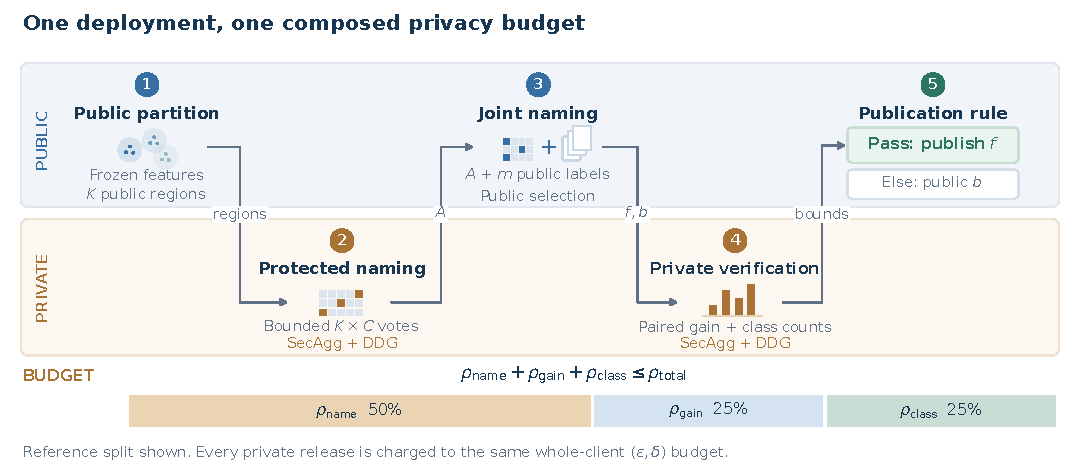
\includegraphics[width=.9\textwidth,trim=0 .19in 0 .40in,clip]{figures/fig-privacy-pipeline.pdf}
\Description{Public and private lanes of one deployment: public partition,
protected naming, joint naming, private verification and the publication
rule, with all private releases charged to one composed budget.}
\caption{One deployment across public and private operations. Protected
naming (2) and verification (4) consume the same whole-client privacy budget;
all operations on released statistics are public post-processing. Release
objects (regional votes, clipped head, pooled per-example votes) differ only
in step 2. The reference $50/25/25$ split is shown; other allocations change
the shares, not the composition rule.}
\label{fig:pipeline}
\end{figure*}



\subsection{A public partition for knowledge reuse}
\label{sec:method:cluster}

A fixed public extractor $g$ and public $K$-means form nonempty regions
$P_1,\ldots,P_K$, shared across rounds independently of private data.
Singleton regions recover per-example transfer; random partitions share the
sensitivity, so matched controls test geometry.

\subsection{One bounded opinion per region}
\label{sec:method:report}

For client model $f_i$, the regional posterior is
\begin{equation}
\bar R_i[k,\cdot]=\frac1{|P_k|}\sum_{x\in P_k}f_i(x)
\in\Delta^{C-1}.\label{eq:report}
\end{equation}
M votes for the largest component of $\bar R_i[k,\cdot]$.
R votes on $f_i(x_k^*)$, where $x_k^*$ is the public point nearest the
centroid: public representative queries followed by regional label propagation.
Both emit K one-hot rows over identical regions, matching sensitivity,
payload and partition quality.

\subsection{Noisy consensus and local learning}
\label{sec:method:agg}

Each client adds independent integer discrete-Gaussian shares to its quantised
report. The aggregate-only layer exposes $S=\sum_i(sR_i+G_i)$, and the server
projects $S/(sn)$ row-wise onto the simplex to obtain $A$.
For ordinary consensus, the target is
\begin{equation}
\hat y(x)=\arg\max_c A[k(x),c].\label{eq:targets}
\end{equation}
Centered decoding uses a fixed class-prior correction: with public region weights
$w_k=|P_k|$, subtract
$\pi_c=\sum_k w_k A[k,c]/\sum_k w_k$ before taking the arg-max.
It counters a common class preference under narrow local label coverage and
is the fixed zero-label decoder. Raw and coverage decoding are separate post-processing rules of the
same matrix; counted public labels can choose their use in joint naming.

\paragraph{Coverage-constrained decoding}
At taxonomy resolution $K=C$, a prespecified alternative is a one-to-one
assignment using the released matrix:
\begin{equation}
\hat\pi=\arg\max_{\pi\in\mathfrak S_C}\sum_k |P_k|A[k,\pi(k)],
\qquad \hat y(x)=\hat\pi(k(x)).
\label{eq:matching}
\end{equation}
Hungarian assignment solves it; it guarantees class coverage, while
correctness depends on whether the public regions support a one-to-one class
allocation. It needs no further private query or budget.
Soft-target controls reuse this protected matrix and are separately indexed.

The primary $T=1$ protocol trains each client privately before a single
release. We compare 60 and 180 pre-release SGD steps without proxy targets.
The naming-only contrasts allocate the full budget to this release;
Section~\ref{sec:private-verification} allocates part to private verification.
The $T=3$ extension trains for 60 steps before each release, mixing equal
private/proxy halves after the first. Releases 1/2 supervise later rounds;
release 3 follows the final local fit. All three consume budget. The extension couples later teachers to earlier names. A private-only
three-release control separates that feedback path from post-release averaging.

\paragraph{Two readouts from the same release}
The public classifier predicts
$\hat y(x)=\hat y_{\arg\min_k\|g(x)-\mu_k\|_2}$ using released regional
labels and fixed public centroids, post-processing publishable under the
transcript's whole-client DP; client models are not published. An optional
public softmax student trains for 180 server steps on the protected labels
only, with its public compute reported separately.

\paragraph{Payload and computation}
At $|P|=2000$, $C=10$, a $K=10/20$ release uses $100/200$ integer
coordinates, versus $20000$ per-example and $1280$ head coordinates, before
secret-sharing overhead. All server work after the release is public
post-processing. Row-wise
simplex projection of the $K\times C$ matrix costs $O(KC\log C)$ by
sorting; centered decoding costs $O(KC)$; the coverage-constrained and joint
decoders solve one $C\times C$ assignment in $O(C^3)$ time by the Hungarian
method. Exact LOO for joint assignment needs at most $C+1$ assignment solves
per weight (Proposition~\ref{prop:loo}), independent of $m$. Server cost thus
scales with $K$ and $C$, not with private data size.

Taxonomy resolution $K=C$, M and centered decoding specify the main
condition without public task labels; larger K and full-label configurations
are separate conditions.

\section{Privacy Model and Analysis}
\label{sec:threat}
\label{sec:threat:setting}

\subsection{Protected aggregate and whole-run client privacy}

A fixed cohort of $n$ clients participates in each of $T$ rounds. Replace-one
adjacency changes the entire dataset of one honest client. Public features,
partitions and configurations are independent of private datasets. The
server's entire view of client data is a sequence of protected sums and
broadcasts; local models, reports and honest noise shares stay hidden.

\paragraph{Aggregation assumptions}
A1: secure additive aggregation reveals the sum and metadata that is public or
independent of protected data. A2: at most $t<n$ contributors disclose reports
and noise to the server, leaving $h=n-t$ honest independent shares.
A3: aggregation parties preserve that view against the stated coalition.
A4: honest contributors use bounded reports and fresh independent noise;
participation is fixed ($q=1$), with recalibration or abort if the required
honest cohort is unavailable. Secret-sharing or split-and-mix protocols can
instantiate the interface~\cite{bonawitz2017practical,corriganGibbs2017prio,ishai2006cryptography};
experiments implement protected-sum arithmetic.

\begin{table}[t]
\caption{Release Interfaces under Replace-One Client Adjacency}
\label{tab:release-interfaces}\small
\centering
\begin{tabular}{@{}lcc@{}}\toprule
released object & coordinates & $L_2$ sensitivity \\\midrule
clipped parameter update & $d_{\mathrm{model}}$ & $2B$ \\
joint per-example votes & $|P|C$ & $\sqrt{2|P|}$ \\
public-region votes & $KC$ & $\sqrt{2K}$ \\
\bottomrule\end{tabular}
\end{table}

\subsection{Sensitivity of the release objects}

Table~\ref{tab:release-interfaces} compares clipping (norm $B$) and release
resolution before quantisation and transport sharing;
the compact head shares $128$-dimensional features, while regional naming
keeps each client's parameters local.

\begin{lemma}[Report sensitivity]
\label{lem:sens}
For $R,R'\in(\Delta^{C-1})^K$, $\|R-R'\|_2\le\sqrt{2K}$,
with equality for opposing one-hot rows. This holds for every public partition.
\end{lemma}

\begin{lemma}[Integer sensitivity]
\label{lem:sens-int}
One-hot reports have $\Delta_q=s\sqrt{2K}$ exactly.
Rounded posteriors have $\Delta_q\le s\sqrt{2K}+\sqrt{KC}$.
A parameter update clipped at $B$ and guarded after rounding in the integer
ball $L_B=\lceil sB+\sqrt d/2\rceil$ has $\Delta_q\le2L_B$.
\end{lemma}

Both follow because simplex rows differ in squared norm by at most two and
rounding adds at most $\sqrt{KC}$; a guarded head lies in an integer ball of
diameter $2L_B$.

\subsection{Release mechanism and accounting}

\paragraph{Release}
Each client submits shares of $sR_i+G_i$ modulo $2^{64}$, with
$s=2^{16}$ and independent coordinates
$G_i[j]\sim\mathcal N_{\mathbb Z}(0,b^2)$.
Noise is drawn by exact rejection sampling \cite{canonne2020discrete}, so the
analysis applies to the sampled distribution, not a floating-point
approximation.

\begin{theorem}[One protected aggregate]
\label{thm:round}
Under A1--A4, the aggregate in dimension $d$ is $\rho_r$-zCDP, where
\begin{equation}
\rho_r=\frac{\Delta_q^2}{2hb^2}+d\,\tau_h(b),
\quad \tau_h(b)\le10(h-1)e^{-\pi^2b^2}.
\label{eq:round-rho}
\end{equation}
For $h=1$, $\tau_h=0$. The bound needs $b\ge1/2$; every recorded release has
$b\ge\MinNoiseScale{}$.
\end{theorem}

After disclosed coalition shares are subtracted, $h$ honest shares remain,
and Kairouz et al.~\cite[Prop.~14, full version]{kairouz2021distributed} give
$\rho_r$ with $\tau_h=10\sum_{k<h}e^{-2\pi^2b^2k/(k+1)}$, which
$k/(k+1)\ge\frac12$ bounds as in Eq.~\eqref{eq:round-rho}; modular addition, projection, matching and
soft-target construction are post-processing.

\begin{theorem}[Adaptive whole run]
\label{thm:run}
Conditionally calibrated releases compose to
$\rho_{\mathrm{total}}\le\sum_{r=1}^T\rho_r$.
The complete server transcript is $(\varepsilon,\delta)$-DP whenever
\begin{equation}
\rho_{\mathrm{total}}+2\sqrt{\rho_{\mathrm{total}}\log(1/\delta)}
\le\varepsilon.
\label{eq:accounting}
\end{equation}
\end{theorem}

Conditioning on data-independent random tapes and each preceding public
transcript fixes the other clients' responses while the replaced report
stays bounded, so adaptive zCDP composition covers every
broadcast~\cite{bun2016concentrated}.

Test metrics and clean-count diagnostics are offline measurements,
outside the deployment transcript claimed to satisfy this guarantee.
Verification releases in Section~\ref{sec:private-verification} are further
rounds of the same transcript and compose under Theorem~\ref{thm:run}.

\subsection{Integer calibration and numerical certificates}

Writing $L=\log(1/\delta)$ and
$\rho_\varepsilon=(\sqrt{L+\varepsilon}-\sqrt L)^2$, the total target is
$\rho_\varepsilon$; for each per-release share $\rho_j$ we use
\begin{equation}
b_j=\left\lfloor\Delta_{q,j}/\sqrt{2h\rho_j}\right\rfloor+1,
\label{eq:integer-scale}
\end{equation}
and verify $\Delta_{q,j}^2/(2hb_j^2)+d_j\tau_h\le\rho_j$. In every
recorded release $\tau_h<10^{\TauMaxLog}$, below the $10^{-30}/4$ the
accountant charges, so all \TauCerts{} recorded certificates hold with this
constant (artifact check).
All budgets are recomposed with 90-digit arithmetic, and a union bound
certifies modulo-$2^{64}$ wrap probability below $10^{-30}$ per release.

Every release keeps a certificate with actual $n$, honest $h$, integer
sensitivity, noise scale and composed budget. For $t=0$, mean-noise standard deviation is bounded by
\begin{equation}
v=\frac{b\sqrt n}{sn}\approx\frac{\sqrt{TK/\rho_\varepsilon}}{n}.
\label{eq:design-budget}
\end{equation}
Noise grows with $\sqrt{TK}$ and shrinks with $n$, so resolution, release
count and cohort size can be traded before any private data are touched.

\section{Label Budgets, Joint Naming and Verification}
\label{sec:quality}

\subsection{Annotation resources and joint naming}

$L_m$ holds the m labelled development examples of Section~\ref{sec:problem};
test queries are inductive and outside training graphs.

Fourteen public learners include regional majority, three assignment variants
(differing in how empty regions are treated), class centroids, five ridge
heads and four graph propagation configurations \cite{zhou2003consistency}
with two strengths, with/without class-mass normalization. Ridge and graph
learners use exact LOO predictions; a fixed public-first order resolves ties.
Web selection uses observed-class balanced accuracy.

With observed regional label counts $L[k,c]$, projected private matrix A and
public region sizes $w_k$, joint naming solves
\begin{equation}
\hat\pi_\lambda=\arg\max_{\pi\in\mathfrak S_C}
\sum_k\left\{L[k,\pi(k)]+\lambda\frac{w_k}{\bar w}A[k,\pi(k)]\right\}.
\label{eq:fusion}
\end{equation}
Here $K=C$, $\bar w=\sum_k w_k/K$ and
$\lambda\in\{.01,.03,.1,.3,1,3,10,30\}$. LOO selects among the fourteen
public learners, joint assignments and fixed private centered/coverage rules.
All candidates reuse one protected matrix, so selection adds no private
query. Exact LOO is efficient for the assignment candidates.

\begin{valueprop}[LOO on matched edges]
\label{prop:loo}
For $S=L+\lambda\operatorname{diag}(w/\bar w)A$, let $\pi$ maximize assignment
weight. Removing an example on an unmatched edge $(k,c)$, $c\ne\pi(k)$,
cannot make that edge correct in the reduced problem. Thus LOO correctness
for all m examples needs at most $C+1$ assignment solves per weight.
\end{valueprop}
Every assignment using an unmatched removed edge loses one unit while the
optimum loses none; examples on one matched edge share one refit.

The same joint decoder receives a protected head's mean proxy-region softmax
or point scores averaged inside each region before projection. Native head
prediction is an additional fixed head-arm candidate.

\subsection{Public evidence and publication targets}

The public augmentation rule requires a positive paired LOO lower gain,
all-class proxy predictions and a positive Wilson-form recall bound per class
(heuristics, since prediction and selection are dependent), else it falls
back to the public model. A missing labelled class forces rejection, so
verification labels also strengthen the public competitor; private
verification changes the source of evidence and charges its privacy.

\subsection{Private verification within one total budget}
\label{sec:private-verification}

After protected naming fixes candidate f and public comparator b, client i
computes held-out gain $d_i=u_i(f)-u_i(b)\in[-1,1]$ and a normalized
$C\times4$ histogram of true class and joint correctness of f and b; both
use distributed discrete-Gaussian shares.

The demonstration fixes $\rho$ fractions $1/2,1/4,1/4$ for naming, gain and
class statistics. Conditional composition in Theorem~\ref{thm:run} charges
all three releases to the same total $(\varepsilon,10^{-5})$ budget.
With released mean $\tilde r$ and gain-channel mean-noise proxy $v_g$, set
\begin{equation}
\underline G=2\tilde r-1
-2v_g\sqrt{2\log(1/\alpha_g)}-s^{-1}.
\label{eq:private-gain-bound}
\end{equation}
Discrete-Gaussian sub-Gaussian tails \cite{canonne2020discrete} imply
$\Pr(\underline G>G)\le\alpha_g$, where $G=n^{-1}\sum_i d_i$.
Direct histogram numerator/denominator bands yield simultaneous class-recall lower
bounds (Proposition~\ref{prop:private-validation} below). We fix
$\alpha_g=\alpha_h=.025$: gain-only acceptance uses $\underline G>0$;
class-checked acceptance also requires every recall lower bound positive. A
\emph{false accept} is an accepted case whose clean held-out statistics miss
the target ($G\le0$, or some class recall zero or below the threshold).
Rejection returns the public comparator without certifying its class
recall. Coverage concerns validation noise and the finite held-out cohort,
not unseen clients; publishing or rejecting is post-processing.

\paragraph{Bounded validation reports}
In the cost ladder each client has 120 held-out records. For paired gain, encode
$q_i=\operatorname{round}(s(1+d_i)/2)\in[0,s]$. Its integer sensitivity
is s, and converting the rounded mean to gain adds at most $1/s$ error.
The class report $h_i\in\Delta^{4C-1}$ records true class and joint binary
correctness $(a,b)$ of candidate/comparator. Largest-remainder rounding
gives $Q_i\ge0$, $\sum Q_i=s$, with coordinate error below $1/s$.
Its integer squared sensitivity is exactly $2s^2$. Both reports have fixed
dimension (1 and $4C$), independent of the number of held-out records.

\begin{valueprop}[Conditional finite-heldout coverage]
\label{prop:private-validation}
Assume the specified reports and independent noise shares. Fix the naming
transcript, public labels and actual held-out cohort.
Equation~\eqref{eq:private-gain-bound} has one-sided coverage at least
$1-\alpha_g$. Let $z=\sqrt{2\log(4C/\alpha_h)}$ and define
\begin{equation}
a_N=\sqrt2v_h z+2/s,\qquad a_D=2v_h z+4/s.
\label{eq:hist-radius}
\end{equation}
For released normalized histogram $\tilde h$, take
$D_c^U=\min(1,[\sum_{a,b}\tilde h_{c,ab}+a_D]_+)$ and
$N_c^L=[\tilde h_{c,10}+\tilde h_{c,11}-a_N]_+$.
The clipped ratio $N_c^L/D_c^U$ is simultaneously a recall lower bound for
all classes with probability at least $1-\alpha_h$, taking zero if $D_c^U=0$.
Joint gain/class coverage is at least $1-\alpha_g-\alpha_h$, apart from
the stated wrap term.
\end{valueprop}
\begin{proof}[Proof sketch]
Each exact share is sub-Gaussian with proxy $b$ (Lemma~16 of
Canonne et al.~\cite{canonne2020discrete}), so the mean has proxy $v$; a
correct-mass sum has proxy $\sqrt2v_h$ and a class mass $2v_h$. A union over
the $2C$ fixed linear targets with rounding errors gives
Eq.~\eqref{eq:hist-radius}, and monotone division plus a union with the gain
event completes the claim.
\end{proof}

This is noise coverage for a finite cohort, not a posterior probability
given acceptance. Whole-client adjacency affects training and held-out
records, so all releases compose sequentially.

\paragraph{Why targets differ in cost}
The gain target resolves one scalar with multiplier
$\sqrt{2\log(1/\alpha_g)}$; classwise targets resolve $2C$ simultaneous
bands with the larger $z$, and each must separate from zero a class mass of
order $1/C$. Section~\ref{sec:eval:verification} measures the resulting
cost ladder.

Higher K can raise purity while increasing the noise in
Eq.~\eqref{eq:design-budget}; natural writers test this.

\section{Experimental Evaluation}
\label{sec:eval}

The evaluation follows the platform's three decisions (Q1--Q3), then
explains where regional value is lost; every comparison states its resource
vector.

\subsection{Tasks, resources and replication}
\label{sec:eval:setup}

\begin{table}[t]
\caption{Evaluated Settings}
\label{tab:setup}\small\setlength{\tabcolsep}{2pt}
\centering
\begin{tabular}{@{}lrlllll@{}}\toprule
Task & $C$ & Features & Private & $n$ & $\varepsilon$ & Splits \\
\midrule
CIFAR & 10 & DINOv2/128 & 45000 img. & 1k, 10k & .1 & 2000/5000/4033 \\
MNIST & 10 & DINOv2/128 & 53000 img. & 10k & .1 & 2000/5000/5000 \\
Usenet & 6 & TF-IDF/128 & 4249 authors & 3k & 1 & 1500/1500/1737 \\
FEMNIST & 62 & DINOv2/128 & 2600 writers & 1k, 2k & .1, 1 & 2000/5000/4549 \\
Verif. & 10 & DINOv2/128 & 480/120 rec. & 1k & .1, 1, 3 & as CIFAR \\
\bottomrule\end{tabular}
\end{table}

\begin{table}[t]
\caption{Study Designs}
\label{tab:studies}\small\setlength{\tabcolsep}{2pt}
\centering
\begin{tabular}{@{}>{\raggedright\arraybackslash}p{.28\columnwidth}>{\raggedright\arraybackslash}p{.34\columnwidth}>{\raggedright\arraybackslash}p{.15\columnwidth}>{\raggedright\arraybackslash}p{.15\columnwidth}@{}}\toprule
Study (§) & Cohorts $\times$ label draws & Frozen first & Reported \\\midrule
Label access, interfaces (B, C) & 10 protocol + 10 confirmation cohorts $\times$ 100 & design & Tab.~\ref{tab:joint-controls}, Figs.~\ref{fig:label-frontier}, \ref{fig:value-mechanisms} \\
Weaker encoder (B) & CIFAR-1k confirmation cohorts & design & text \\
Cost ladder (D) & 10 cohorts $\times$ 100 $\times$ 3 $\varepsilon$ (3000) & split, targets & Tab.~\ref{tab:verify-ladder} \\
Protocol price (D) & ladder cohorts, draws 50--99 & Opt.\ post hoc & Tab.~\ref{tab:cost} \\
Source-disjoint (D) & 10 new cohorts $\times$ 100 & design & Tab.~\ref{tab:cost} \\
Split, CIFAR (D) & 10 + 10 cohorts, disjoint sources (\BCCases{}) & design, split & Tab.~\ref{tab:budgetconf} \\
Split, FEMNIST (D) & 10 + 10 cohorts, disjoint writers (\FCCases{}) & split, planner & text \\
Gated + verified (E) & 10 new cohorts per task (\VTCases{}) & design & Tab.~\ref{tab:verify-teacher} \\
Ceilings (E) & clean votes of label-access cohorts & offline & Tab.~\ref{tab:decomposition}, Fig.~\ref{fig:ceiling} \\
\bottomrule\end{tabular}
\end{table}

Table~\ref{tab:setup} lists the settings (features: encoder/proxy-fitted
dimension; splits: proxy/development/test) and Table~\ref{tab:studies} the
studies, their cohorts and what each froze before its outcomes. Images use frozen DINOv2
ViT-S/14 features \cite{oquab2023dinov2} and Usenet public TF-IDF, each
reduced by proxy-fitted PCA/SVD and row-normalized. Constructed image
clients draw 600 images with replacement under Dirichlet $\alpha=.1$; the
protected unit is a complete constructed reporting dataset, and source copies
at other clients remain in the adjacent database. Usenet clients are
From-header authors over six content families, with headers and quotes
removed, disjoint authors per split, and balanced accuracy as metric.
Official 62-class FEMNIST \cite{caldas2018leaf,tff2024emnist} assigns
distinct writers, with their original records, to private, public and test
roles. All recalls are recorded. These task labels can be supplied by public
annotators; no claim of irreplaceable private Web semantics follows.

\paragraph{Protocols and phases}
The artifact lists all cohort phases and seeds. Softmax learners use
batch 128, learning rate .1, momentum .9 and weight decay $5\times10^{-4}$.
Naming-only T=1 releases once after 60/180 private steps; feedback T=3
uses 60 steps before each release. All set $\delta=10^{-5}$ with equal
actual/calibrated populations. Heads fix clipping at $B=1$ without task
labels.

For $m/C\in\{1,3,5,10,20,50\}$, random acquisition has 100 nested label
draws; CIFAR/MNIST balanced acquisition has 50 draws. Feature-directed
annotation selects q nearest development points per public region before
revealing labels, filling shortages by nearest-to-assigned-centroid points.
Each set crosses ten cohort/noise seeds. A two-way bootstrap (2000
resamples) resamples label draws and cohorts; simultaneous public gain
intervals cover all six budgets and fourteen public learners.

\paragraph{Implementation and reproducibility}
Graphs use 20 neighbors and $\alpha=.8/.95$; ridge uses
$.001$--$10$; k-means uses five starts and seed 1729.
Research noise keys and clean diagnostics are outside the deployment
transcript; one GPU computes the protected-sum arithmetic, not
secure-aggregation performance. Cases sharing cohorts and label sets are not
independent trials. The artifact maps every table and figure to its records; \texttt{verify} re-aggregates
them and re-checks every budget certificate, and \texttt{smoke} retrains
cohorts and reproduces their protected outputs and decisions.

\begin{table*}[t]
\caption{Equal-Label Comparison of Release Interfaces}
\label{tab:joint-controls}\small
\centering
\begin{tabular}{@{}llrrrrr@{}}\toprule
Task, clients / $\varepsilon$ & Group & Public & Region joint & Head joint & Point joint & Native Head \\
\midrule
CIFAR 1k / 0.1 & I & 61.6 & 74.6 & 76.6 & 76.9 & 34.3 \\
CIFAR 10k / 0.1 & I & 61.6 & 87.4 & 91.1 & 87.4 & 94.0 \\
MNIST 10k / 0.1 & I & 46.2 & 44.4 & 72.2 & 44.7 & 77.0 \\
Usenet 3k / 1 & P & 32.1 & 28.2 & 31.8 & 28.9 & 23.2 \\
FEMNIST 1k / 0.1 & P & 37.3 & 36.0 & 36.0 & 36.0 & 12.1 \\
FEMNIST 1k / 1 & P & 37.3 & 35.9 & 38.1 & 36.0 & 40.7 \\
FEMNIST 2k / 0.1 & P & 37.3 & 36.0 & 35.9 & 36.0 & 26.3 \\
FEMNIST 2k / 1 & P & 37.3 & 35.8 & 38.5 & 36.1 & 41.3 \\
\bottomrule\end{tabular}
\end{table*}


\begin{figure*}[t]
\centering
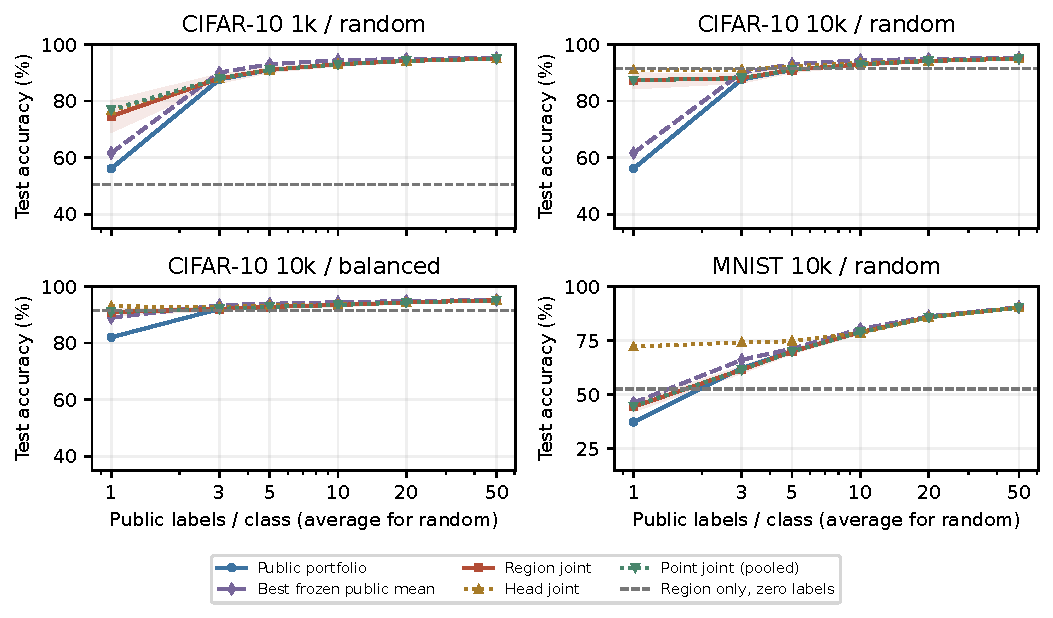
\includegraphics[width=.72\textwidth]{figures/fig-joint-frontier.pdf}
\Description{Matched public label budgets under random and balanced acquisition,
with public learning and identically decoded private release objects.}
\caption{Label access changes the comparison. Random panels use independent
confirmation cohorts/labels; balanced uses protocol cohorts. All private
arms release once at $\varepsilon=.1$ after 180 private steps. Public envelope
is descriptive over fourteen frozen learners; the portfolio is a LOO rule.
Private joint curves are ungated. All fitting/selection labels are inside m.
Shading is crossed pointwise bootstrap; text gives simultaneous intervals.}
\label{fig:label-frontier}
\end{figure*}

\begin{figure*}[t]
\centering
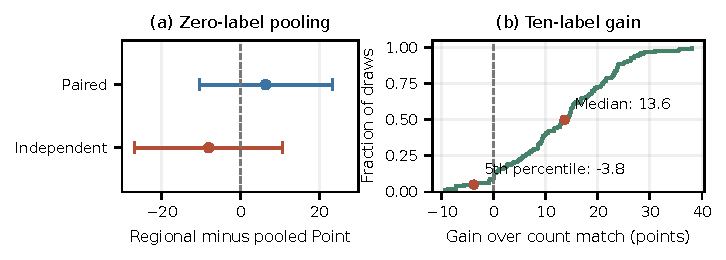
\includegraphics[width=.68\textwidth]{figures/fig-value-mechanisms-print.pdf}
\Description{Zero-label regional-minus-pooled differences reverse across two
cohort groups; ten-label gains have a positive median and a negative lower tail.}
\caption{CIFAR-1k, $\varepsilon=.1$. (a) Zero-label centered NN: regional/pooled
Point means are $52.2/45.8\%$ in paired cohorts and $50.3/58.4\%$ in independent
cohorts. Paired Student intervals use ten seeds per group. (b) Each label-mean
gain averages ten independent-confirmation cohorts against fixed raw-count
public matching. The 100 draws have mean \JointGain{}, median \GainMedian{}
and fifth percentile \GainFifth{} points. Crossed cases are not independent.}
\label{fig:value-mechanisms}
\end{figure*}

\subsection{What to buy: annotation access and the gain distribution}
\label{sec:eval:main}
\label{sec:eval:frontier}

With balanced labels (50 draws; the artifact tabulates all fourteen public
learners), three supplied
labels per class name the fixed CIFAR partition at $91.59\%$ in all 50 draws
(graph propagation: $92.61\%$), and ten feature-directed annotations recover
the same classifier without private reports. On MNIST's less class-aligned
regions one label per class gives $38.28\%$ majority naming versus
$58.36\%$ graph propagation.

Under passive random access, independent CIFAR-1k with ten labels gives
$61.62\%$ for the strongest mean public learner (raw-count matching) and
$74.62\%$ for joint naming (Figure~\ref{fig:label-frontier}). The
\JointGain{}-point mean gain has simultaneous interval \JointGainCI{}. The
median label-mean gain is \GainMedian{} points, so a few large draws do not
drive it; its fifth percentile is \GainFifth{}, and \GainNegativeDraws{}\% of
label means and \GainNegativeCases{}\% of label/cohort cases are negative
(Figure~\ref{fig:value-mechanisms}(b)). Label- and cohort-mean SDs are
\LabelAxisSD{}/\CohortAxisSD{} points.

Every ten-label CIFAR draw omits a class (30/50 labels: $31/7\%$), and the
public class-check rule rejects private augmentation at every tested budget,
so $74.62\%$ is an ungated utility (the artifact tabulates all fallbacks).
Random-only access is an experimental contract, not a known constraint of
CIFAR or Usenet. LOO selection contributes its own variation: the public
portfolio gives $56.13\%$ versus fixed count matching's $61.62\%$, and at
CIFAR-10k joint selection gives $87.35\%$ versus fixed zero-label private
naming's $91.59\%$ (Section~\ref{sec:eval:ceiling}).

\paragraph{A weaker encoder}
A frozen design replaces DINOv2 by an ImageNet ResNet-18 and reruns the
independent CIFAR-1k comparison with the same images, cohorts, label draws,
learners and release. The partition ceilings fall to
\EncCeilOne{}/\EncCeilMany{}\%. Ten feature-directed labels again reach the
one-to-one ceiling without private reports (\EncDirected{}\%); with ten
random labels, joint naming (\EncJoint{}\%) changes the strongest public
learner (\EncPublic{}\%) by \EncGain{} points (\EncGainCI{}). The registered
E1, a positive passive-access gain, fails; E2, directed labels beating random
labels plus private reports, holds. Under both encoders acquisition decides
whether private reports are needed; their passive-access value also needs
regions that carry the classes (Section~\ref{sec:eval:ceiling}).

\subsection{What to release: sensitivity versus accuracy}
\label{sec:eval:rounds}

Per-example votes are $\sqrt{|P|/K}$ times more sensitive than regional
reports (Section~\ref{sec:threat}); at $|P|=2000$ and $K=10$ the factor is
about 14, and they carry 20000 rather than 100 coordinates per client,
against 1280 for a head. Table~\ref{tab:joint-controls} holds
post-processing fixed: all three objects feed the same joint decoder and LOO
selection with the same labels (I/P: independent/paired cohorts; Public:
strongest of the fourteen public learners; Native Head uses no labels). Pooled point and regional joint naming differ
by at most \PointRegionMaxGap{} points on all \PointRegionSettings{} settings
(CIFAR-1k: $76.94$ versus $74.62\%$), while the head, whose native
predictions the partition does not bound, wins where the partition limits
regional naming (MNIST-10k: \HeadMnistTenK{} versus \RegionMnistTenK{}\%; at
CIFAR-10k native Head gives $94.0\%$). Published designs run through the same
protected sum in the inherited three-release protocol ($10^4$ clients,
$\varepsilon=.1$, \ExtSeeds{} seeds, publicly configured settings): on
CIFAR-10, DP-FedCT's per-example votes, our Point interface, reach
\ExtFedCTCifar{}\% and PATE-DI's screened teacher votes (RDP conversion)
\ExtPATECifar{}\%, against \ExtSDDCifar{}\% for regional reports and
\ExtHeadCifar{}\% for the clipped DP-Head (MNIST: \ExtFedCTMnist{},
\ExtPATEMnist{}, \ExtSDDMnist{} and \ExtHeadMnist{}\%).

Pooling explains why the sensitivity gap does not reach accuracy. Relative
to regional noise, averaging independent point noise in
region k has standard-deviation ratio approximately
\begin{equation}
\frac{v_{\mathrm{point,pool},k}}{v_{\mathrm{region}}}
\simeq\sqrt{\frac{|P|}{K |P_k|}}.
\label{eq:pooling-ratio}
\end{equation}
CIFAR's region sizes give ratios .88--1.07: pooled point votes carry about the
regional noise. At zero labels, CIFAR-1k regional-minus-pooled paired
differences are $+6.39$ points ($[-10.48,23.26]$) in protocol cohorts and
$-8.02$ ($[-26.81,10.77]$) in independent cohorts
(Figure~\ref{fig:value-mechanisms}(a)); neither supports a stable regional
advantage. The $\sqrt{|P|/K}$ ratio is a payload and interface property, not
an accuracy guarantee.

With fixed 60-step teachers, T=1 raises CIFAR-1k from $26.86\%$ to
$49.56\%$; no-feedback T=3 controls show no universal feedback penalty. The
pooling, round and no-feedback tables are in the artifact.

\subsection{What evidence to buy: mean gain versus class evidence}
\label{sec:eval:verification}

The verification demonstration (Table~\ref{tab:setup}, Verif.) uses ten new
CIFAR-1k cohorts, 100 fresh ten-label draws and an 80/20 source split
between training and held-out records. The comparator is raw-count matching;
candidates (eight joint weights, fixed private and public count rules) are
chosen from protected naming and the ten labels. Each of the 3000 cases
charges all three releases to one total budget; every utility is
unconditional, a rejection scoring its public fallback.

\paragraph{A cost ladder of publication targets}
Table~\ref{tab:verify-ladder} evaluates practical targets on these protected
outputs (acceptance / unconditional test accuracy; each row is a separately
declared rule with its own $\alpha=.025$ class family). Gain-only acceptance is \TightGlobalAccept{}\% at $\varepsilon=.1$
and \MiddleGlobalAccept{}\% at $\varepsilon=1$, where direct class-sum bounds
accept \MiddleClassAccept{}\% (initial coordinate-wise bands: zero). At $\varepsilon=3$, class-checked acceptance reaches
\LargerClassAccept{}\% ($86.63\%$ test accuracy against $62.30\%$ public), a
budgeted route to classwise evidence, not a validation of the $74.62\%$
classifier at unchanged privacy. A mean gain of at least $.20$ still accepts
\LadderGainTwoTenth{}\% of cases at $\varepsilon=1$. All-class recall of at
least $.25$ is accepted in \LadderRecallQuarterThree{}\% of cases at
$\varepsilon=3$, and $.50$ at no tested budget. Per-class non-degradation
against the comparator, $\mathrm{recall}_{f,c}-\mathrm{recall}_{b,c}\ge-\eta$,
depends on its tolerance: at $\varepsilon=3$ it accepts
\LadderNondegQuarter{}\% at $\eta=.25$ but \LadderNondegHalf{}\% at
$\eta=.5$; its band radius must fall below $\eta$ times a class mass of order
$1/C$. Costs are ordered only for stated thresholds. Gain-policy false accepts are 1/1000 at $\varepsilon=.1$, and no ladder rule
records one at $\varepsilon\ge1$.

\paragraph{What the cheap target publishes}
A correct mean-gain certificate says nothing about the worst class
(Figure~\ref{fig:verification}(a)). At $\varepsilon=1$ the mean-gain rule
publishes \MinRecGainOnePub{} of 1000 cases; \MinRecGainOneZero{}\% of them
recall some class below $1\%$ and \MinRecGainOneTenth{}\% below $10\%$
(\MinRecGainThreeTenth{}\% at $\varepsilon=3$). Every classifier the
all-recall rule publishes recalls each class above $50\%$; the ladder's price
difference buys exactly this tail.

\begin{table}[t]
\caption{Verification-Cost Ladder of Publication Targets}
\label{tab:verify-ladder}\small
\centering
\begin{tabular}{@{}lrrr@{}}\toprule
Publication target & $\varepsilon=.1$ & $\varepsilon=1$ & $\varepsilon=3$ \\
\midrule
gain $>0$ & 4.6 / 63.7 & 86.8 / 88.9 & 87.0 / 88.9 \\
gain $\ge.10$ & 2.2 / 63.0 & 82.0 / 88.2 & 85.0 / 88.7 \\
gain $\ge.20$ & 0.7 / 62.6 & 58.2 / 83.4 & 64.6 / 85.1 \\
all recalls $>0$ & 0.0 / 62.3 & 6.2 / 64.3 & 75.9 / 86.6 \\
all recalls $\ge.25$ & 0.0 / 62.3 & 0.0 / 62.3 & 75.7 / 86.6 \\
all recalls $\ge.50$ & 0.0 / 62.3 & 0.0 / 62.3 & 0.0 / 62.3 \\
non-degr. $\eta=.25$ & 0.0 / 62.3 & 0.0 / 62.3 & 2.0 / 63.2 \\
non-degr. $\eta=.50$ & 0.0 / 62.3 & 0.0 / 62.3 & 83.1 / 87.8 \\
\bottomrule\end{tabular}
\end{table}


\paragraph{Protocol price versus target price}
The ladder fixes one protocol: a $50/25/25$ split, both reports released and
two-sided bands. Table~\ref{tab:cost} varies each choice on draws 50--99.
\emph{Tight} applies one-sided lower bands to the same histograms (all-recall
acceptance at $\varepsilon=1$: \CostFixedRecallOne{}\% to
\CostTightRecallOne{}\%, nothing else changes); \emph{Re-rel.} re-releases
the stored clean statistics with fresh exact noise after reconstructing all
3000 histograms bit for bit; \emph{Opt.} uses the naming share $\phi$ that
maximized offline test accuracy on draws 0--49 (gain: $\phi$ to naming, the
rest to the gain report; classes: the gain report takes a quarter of the
rest). Both phases score the same test set and cohorts, so \emph{Opt.} is a
retrospective sensitivity analysis: the fixed split is far from best for class
targets ($\phi=\CostOptRecallOnePhi$: \CostRefRecallOne{}\% to
\CostOptRecallOne{}\% at $\varepsilon=1$), so Table~\ref{tab:verify-ladder}
prices one protocol, not the targets.

\begin{table}[t]
\caption{Verification Cost under Four Protocols}
\label{tab:cost}\small\setlength{\tabcolsep}{1.6pt}
\centering
\begin{tabular}{@{}llrrrrrr@{}}\toprule
Target & $\varepsilon$ & Fixed & Tight & Re-rel. & Opt. & $\phi$ & Disjoint \\
\midrule
gain $>0$ & .1 & 5.4/64.5 & 5.4/64.5 & 6.6/64.6 & 12.4/66.4 & .4 & 5.0/64.2 \\
 & 1 & 88.0/90.3 & 88.0/90.3 & 88.0/90.3 & 88.0/90.2 & .1 & 88.0/90.2 \\
 & 3 & 88.0/90.3 & 88.0/90.3 & 88.0/90.5 & 88.2/90.5 & .5 & 88.4/90.6 \\
all recalls $>0$ & .1 & 0.0/62.8 & 0.0/62.8 & 0.0/62.8 & 0.0/62.8 & -- & 0.0/62.8 \\
 & 1 & 6.4/64.9 & 19.8/69.0 & 7.8/65.2 & 81.8/88.5 & .1 & 7.4/65.1 \\
 & 3 & 82.8/89.0 & 82.8/89.0 & 83.6/89.5 & 83.6/89.3 & .3 & 84.2/89.6 \\
all recalls $\ge.50$ & .1 & 0.0/62.8 & 0.0/62.8 & 0.0/62.8 & 0.0/62.8 & -- & 0.0/62.8 \\
 & 1 & 0.0/62.8 & 0.0/62.8 & 0.0/62.8 & 0.0/62.8 & -- & 0.0/62.8 \\
 & 3 & 0.0/62.8 & 0.0/62.8 & 0.0/62.8 & 70.2/85.0 & .1 & 0.0/62.8 \\
\bottomrule\end{tabular}
\end{table}


\paragraph{Choosing the split before deployment}
Can a platform find such a split without the test set? A third frozen
design splits the 45000 private CIFAR images per class into two pools; ten
\emph{development} cohorts come from one and ten \emph{confirmation}
cohorts from the other, each with 1000 clients holding \BCRecTrain{}
training and \BCRecHeld{} held-out records used once. On development cohorts
and label draws 0--49, each target and budget gets the grid $\phi$ that
maximizes the accuracy of the published classifier on the labelled public
validation split; the selection reads only protected decisions and
validation labels and was frozen before any confirmation case ran. Confirmation cohorts, label
draws 50--99 and the test split then compare the frozen share with the fixed
split at the same total budget (Table~\ref{tab:budgetconf},
\BCCases{} cases; $\Delta$ with crossed-bootstrap 95\% interval, FA false
accepts, Best the unused confirmation-best share). The pre-registered primary test holds: at
$\varepsilon=1$, all-recall acceptance rises from \BCFixedRecallOne{}\% to
\BCFrozenRecallOne{}\% ($\BCDiffRecallOneAcc$ points, $\BCDiffRecallOneAccCI$)
and test accuracy from \BCFixedRecallOneUtil{} to \BCFrozenRecallOneUtil{}\%
($\BCDiffRecallOneUtil$, $\BCDiffRecallOneUtilCI$). Recall $\ge.5$ becomes
certifiable at $\varepsilon=3$ (\BCFrozenHalfThree{}\% acceptance,
\BCFrozenHalfThreeUtil{}\% accuracy), mean-gain cells move by at most
\BCGainMaxDiff{} points, and no frozen cell records a false accept.
Development and confirmation curves agree
(Figure~\ref{fig:verification}(b,c)); the frozen share loses at most
\BCMaxRegret{} points to the confirmation-best one. The registered prediction
that class shares fall below $.5$ at $\varepsilon\le1$ failed only where no
share certifies anything and ties default to $.5$. One development cohort
with ten draws already selects well (\BCPilotRecallOne{}\% confirmation
accuracy at $\varepsilon=1$, \BCPilotHalfThree{}\% for recall $\ge.5$ at
$\varepsilon=3$, mean of \BCPilotSubsamples{} such pilots). The pilot is a
separate population with its own ledger: \PilotDevLabels{} development labels
(ten draws of ten), the \PilotValLabels{} public validation labels that score
each published classifier, and \PilotReleases{} protected releases over
\PilotConfigs{} grid configurations. Answered by one population they compose
to \PilotRhoMult{} times a deployment's zCDP budget (total
$\varepsilon\approx\PilotEpsOne{}$ for deployments at $\varepsilon=1$). The
deployment's public learners do not see the pilot's labels; a platform allowed
to train on its validation labels should compare against learners that do.

\paragraph{Natural writers: an external test of the planner}
FEMNIST runs the same protocol (Table~\ref{tab:budgetconf}, lower block):
1000 writers per cohort from two disjoint pools, a seeded 80/20 split of each
writer's records ($H_i$ varies, median 32), 62 random labels, \FCCases{} cases.
Reports, certificates, clean statistics, planner inputs and false-accept
judgments all use the client-weighted statistics of Section~\ref{sec:problem}.
Planner predictions frozen before confirmation lie within \FCPlanGap{} points
of every cell, with no false accept; the cells sit near 0 or 100\%, so this
checks calibration at the extremes. The study prices verification, not
private value: the mean-gain rule accepts \FCGainOne{}\% at $\varepsilon=1$
against the \FCPub{}\% count-matching comparator, yet its \FCUtilFixed{}\%
stays below the strongest public learner on the same labels
(\FCPublicBest{}\%) and \FCTail{}\% of what it publishes recalls some class
below 10\%. Candidates miss whole classes, so no class target is certifiable
and the split cannot help, as the planner predicted.

\begin{table*}[t]
\caption{Budget Split Selected on Development Cohorts and Confirmed on New Cohorts}
\label{tab:budgetconf}\small\setlength{\tabcolsep}{4pt}
\centering
\begin{tabular}{@{}lllrrrrrrr@{}}\toprule
Task & Target & $\varepsilon$ & $\phi$ & Fixed & Frozen & Planner & $\Delta$ accuracy & FA & Best \\
\midrule
CIFAR & gain $>0$ & .1 & .3 & 3.8/63.8 & 4.0/63.8 & -- & +0.0 [$-$1.0, +1.0] & 0 & .5 \\
 &  & 1 & .5 & 88.0/90.2 & 87.6/90.0 & -- & $-$0.1 [$-$0.7, +0.2] & 0 & .6 \\
 &  & 3 & .2 & 88.0/90.6 & 88.0/90.6 & -- & +0.0 [$-$0.2, +0.2] & 0 & .4 \\
 & all recalls $>0$ & .1 & .5 & 0.0/62.8 & 0.0/62.8 & -- & +0.0 [+0.0, +0.0] & 0 & -- \\
 &  & 1 & .2 & 5.4/64.5 & 78.2/87.2 & -- & +22.8 [+18.9, +26.7] & 0 & .3 \\
 &  & 3 & .2 & 83.8/89.6 & 83.6/89.5 & -- & $-$0.1 [$-$0.8, +0.3] & 0 & .6 \\
 & all recalls $\ge.50$ & .1 & .5 & 0.0/62.8 & 0.0/62.8 & -- & +0.0 [+0.0, +0.0] & 0 & -- \\
 &  & 1 & .5 & 0.0/62.8 & 0.0/62.8 & -- & +0.0 [+0.0, +0.0] & 0 & -- \\
 &  & 3 & .1 & 0.0/62.8 & 76.2/87.2 & -- & +24.4 [+19.9, +28.6] & 0 & .1 \\
\midrule
FEMNIST & gain $>0$ & 1 & .9 & 99.0/35.1 & 98.2/35.2 & 98.7/98.1 & +0.0 [$-$0.7, +0.6] & 0 & .7 \\
 &  & 3 & .2 & 100.0/35.5 & 100.0/35.5 & 99.3/99.7 & +0.0 [$-$0.6, +0.5] & 0 & .3 \\
 &  & 10 & .1 & 100.0/35.1 & 100.0/35.1 & 100.0/100.0 & +0.0 [$-$0.2, +0.3] & 0 & .3 \\
 & all recalls $>0$ & 1--10 & .5 & 0.0/11.6 & 0.0/11.6 & 0.0/0.0 & +0.0 [+0.0, +0.0] & 0 & -- \\
 & all recalls $\ge.50$ & 1--10 & .5 & 0.0/11.6 & 0.0/11.6 & 0.0/0.0 & +0.0 [+0.0, +0.0] & 0 & -- \\
\bottomrule\end{tabular}
\end{table*}


\begin{figure*}[t]
\centering
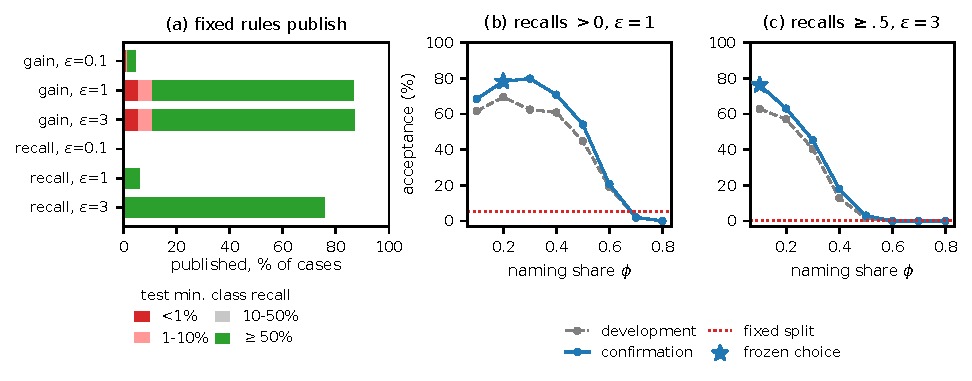
\includegraphics[width=.9\textwidth]{figures/fig-verification-print.pdf}
\Description{Minimum test class recall of classifiers published by the fixed
rules, and development versus confirmation acceptance over the naming share.}
\caption{(a) The 1000 cases per budget of Table~\ref{tab:verify-ladder}, by
the test minimum class recall of the classifier each fixed rule publishes
(offline diagnostic). (b, c) Acceptance over the naming share $\phi$ on the
development cohorts (dashed, used for selection) and the confirmation
cohorts (solid); the star is the frozen choice and the dotted line the fixed
$50/25/25$ split on the confirmation cohorts.}
\label{fig:verification}
\end{figure*}

\paragraph{Source-disjoint clients}
Constructed CIFAR clients in the ladder reuse source images. A design frozen
before implementation rebuilds the ladder on ten new cohorts in which each of
\DisjSources{} private images belongs to one client, \DisjRecords{} for
training and \DisjHeld{} held out, with the same candidates, labels, split and
bands (Table~\ref{tab:cost}, Disjoint). The mean top-class share is \HetDisjoint{}
(last 100 clients \HetLast{}; \HetReused{} with reuse). The gain
policy beats the fallback by \DisjGainImpr{} points at $\varepsilon=1$
(\DisjGainCI{}; \ReusedGainImpr{} with reuse) and every rung stays within
\DisjMaxDiff{} points; the predicted shrinkage did not occur. Its two false
accepts at $\varepsilon=3$ have true gain zero, within $\alpha$.
Disjointness also cuts records per client, so this does not show that
reuse is irrelevant.

\paragraph{A planning map beyond the tested setting}
Per case, the calculator takes the clean gain $g$, class masses $m_c$,
recalls $r_c$ and differences $d_c$. Treating each report as Gaussian with its calibrated std ($2v_g$ for the
gain, $v_h$ per coordinate) and keeping rounding terms, it returns $\Phi((g-a_g-\gamma)/2v_g)\prod_c\Phi(\mu_c/\sigma_c)$,
with $a_g$ the gain band radius. A class rule accepts when a linear statistic
of class $c$ clears zero: for recall $\ge r_0$, $N^L_c-r_0D^U_c\ge0$, so
$\mu_c=r_cm_c-a_N-r_0(m_c+a_D)$ and $\sigma_c=v_h\sqrt{2(1-r_0)^2+2r_0^2}$
(Eq.~\eqref{eq:hist-radius}); for non-degradation, $\mu_c=(d_c+\eta)m_c$
minus its radius and $\sigma_c=v_h\sqrt{2+4\eta^2}$. The linear statistics
ignore the clipping of the bands. Capping $D^U_c$ at 1 can only raise
acceptance and binds only when the released class mass exceeds $1-a_D$
(probability $\Phi((m_c+a_D-1)/2v_h)$); clipping at zero changes a decision
only when that mass falls below $-a_D$. Outside these events the linear form
is exact. Classes and reports multiply because their noise is independent. The
result is an approximate planning quantity, not a coverage guarantee. It reproduces
all \CalcCells{} rates of Table~\ref{tab:verify-ladder} within \CalcGap{}
points; frozen before the new-cohort study of Section~\ref{sec:eval:ceiling},
it also matches its \PlanOOSCells{} gain and class rates (other $n$, $C$ and
natural Usenet clients, class masses \UsenetMassMin{}--\UsenetMassMax{})
within \PlanOOSGap{} points. This validates the noise calibration, not
effect sizes. At the median CIFAR-1k effect sizes, the artifact's planning
map gives the smallest total $\varepsilon$ accepting each target with
probability one half; as $v\propto1/(n\sqrt\rho)$, the
required $\rho$ scales as $n^{-2}$ and $\varepsilon$ roughly as $1/n$. It is
conditional on effect sizes: at $n=10$k it prices all recalls $>0$ at
\PlanRecallZeroNTenK{}, yet the new MNIST candidates, with a nearly empty
worst class, pass in \MnistClassOne{}\% of cases at $\varepsilon=1$.

\subsection{Explaining the losses: partition ceilings}
\label{sec:eval:ceiling}

\begin{table*}[t]
\caption{Where Regional Value Is Lost}
\label{tab:decomposition}\small\setlength{\tabcolsep}{3.2pt}
\centering
\begin{tabular}{@{}lrrrrrrrrrrrrr@{}}\toprule
Task/$\varepsilon$ & Ceil. & Pub. & Room & Clean & Named & Joint & $\Delta_T$ & $\Delta_N$ & $\Delta_S$ & N$\uparrow$ & $v$ & Gated & Head \\
\midrule
CIFAR 1k/0.1 & 91.6/91.6 & 61.6 & +30.0 & 91.6 & 50.3 & 74.6 & +0.0 & +41.2 & -24.3 & 0/10 & 0.215 & 74.6 & 76.6 \\
CIFAR 10k/0.1 & 91.6/91.6 & 61.6 & +30.0 & 91.6 & 91.6 & 87.4 & +0.0 & +0.0 & +4.2 & 0/10 & 0.022 & 91.6 & 91.1 \\
MNIST 10k/0.1 & 52.6/54.1 & 46.2 & +7.9 & 53.9 & 52.6 & 44.4 & +0.2 & +1.3 & +8.2 & 2/10 & 0.022 & 52.6 & 72.2 \\
Usenet 3k/1 & 42.4/42.5 & 32.1 & +10.3 & 32.3 & 20.7 & 28.2 & +10.2 & +11.6 & -7.5 & 0/10 & 0.006 & 21.0 & 31.8 \\
FEMNIST 1k/0.1 & 24.6/42.9 & 37.3 & +5.5 & 35.3 & 7.1 & 36.0 & +7.5 & +28.3 & -28.9 & 0/10 & 0.535 & 36.0 & 36.0 \\
FEMNIST 1k/1 & 24.6/42.9 & 37.3 & +5.5 & 35.3 & 35.5 & 35.9 & +7.5 & -0.2 & -0.4 & 5/10 & 0.055 & 35.9 & 38.1 \\
FEMNIST 2k/0.1 & 24.6/42.9 & 37.3 & +5.5 & 35.3 & 19.8 & 36.0 & +7.5 & +15.5 & -16.2 & 0/10 & 0.268 & 36.0 & 35.9 \\
FEMNIST 2k/1 & 24.6/42.9 & 37.3 & +5.5 & 35.3 & 35.6 & 35.8 & +7.5 & -0.2 & -0.2 & 6/10 & 0.027 & 35.6 & 38.5 \\
\bottomrule\end{tabular}
\end{table*}

% Data figure, generated by export_eab13.py (figures/fig-ceiling-print.pdf): audit panel of the former fig-ceiling;
% its decomposition panel duplicated Table VIII and remains in figures/fig-ceiling.pdf (artifact).
\begin{figure}[t]
\centering
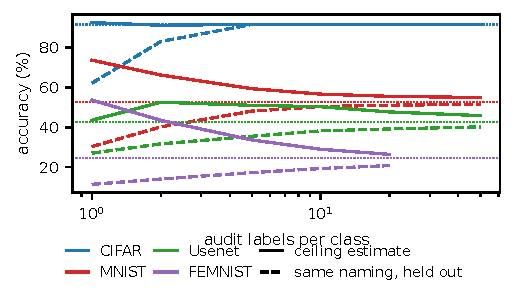
\includegraphics[width=\columnwidth]{figures/fig-ceiling-print.pdf}
\Description{Audit-sample ceiling estimates versus held-out naming accuracy.}
\caption{Auditing the ceiling. A random labelled audit of the development
split: its in-sample one-to-one ceiling estimate (solid) and the test accuracy
of the naming it induces (dashed); dotted lines are the true ceilings; 200
repetitions. Offline diagnostic.}
\label{fig:ceiling}
\end{figure}


A regional readout assigns one class per public region, so its accuracy is
bounded by the \emph{partition ceiling}, the best such assignment within the
decoder's family: $\mathrm{Ceil}_{1:1}$ for
assignment decoders, $\mathrm{Ceil}_{M:1}\ge\mathrm{Ceil}_{1:1}$ for centered
decoding. With $P^\star$ the strongest public learner, the regional part of
the marginal value in Eq.~\eqref{eq:marginal-value} for decoder family $D$
satisfies
\begin{equation}
V^{\mathrm{reg}}_D\le\mathrm{Ceil}_D-P^\star .
\label{eq:ceiling}
\end{equation}
The stored clean vote matrices, never released, make the gap below the
ceiling measurable. Decoding them with the centered decoder of the protected
release gives \emph{noise-free naming} $N_0$; with protected naming
$N_\varepsilon$ and joint selection $J$, on one partition, decoder, data and
seed set,
\begin{equation}
\mathrm{Ceil}_{M:1}-J=\underbrace{\mathrm{Ceil}_{M:1}-N_0}_{\Delta_T}
+\underbrace{N_0-N_\varepsilon}_{\Delta_N}
+\underbrace{N_\varepsilon-J}_{\Delta_S}
\label{eq:decomposition}
\end{equation}
The identity telescopes, so its terms are signed controlled differences, not
causal attributions: noise improves naming on \NoiseImprMnist{} MNIST seeds
and \NoiseImprFemnist{} FEMNIST-2k/1 seeds, and $\Delta_S$ is negative
wherever fusion with the labels corrects noisy names ($\SelCifarOne$ points
on CIFAR-1k). We read $\Delta_T$ as teacher content, $\Delta_N$ as release
noise and $\Delta_S$ as selection only where a term is large and stable
across seeds (Table~\ref{tab:decomposition};
Room is $\mathrm{Ceil}_{M:1}-P^\star$, N$\uparrow$ counts seeds where noise
improves naming, $v$ is the naming-noise std).

\emph{Teacher content} bounds the natural-client tasks. Usenet has
\RoomUsenetMany{} points of room, but noise-free naming reaches only the
public level, \CleanUsenet{}\% ($\Delta_T=\TeachUsenet$): votes barely
differ between regions, so even small noise ($v=\NoiseUsenet$) flips
most regions and costs another \NoiseLossUsenet{} points. On FEMNIST no
assignment decoder can add value (one-to-one ceiling \CeilFemnistOne{}\%,
below public); the many-to-one ceiling leaves \RoomFemnistMany{} points, and
noise-free naming reaches \CleanFemnist{}\% ($\Delta_T=\TeacherFemnist$),
which protected naming matches at $\varepsilon=1$. \emph{Release noise} adds
\NoiseLossFemnistTenth{}--\NoiseLossFemnistOneTenth{} points on FEMNIST at
$\varepsilon=.1$ and \NoiseLossCifarOne{} points on CIFAR-1k
($v=\NoiseCifarOne$), where clean naming is at the ceiling and joint fusion
with ten labels recovers $74.62\%$. \emph{Selection} is the dominant term where
protected naming already realizes the room. On CIFAR-10k ($v=\NoiseCifarTen$)
fixed protected naming reaches the ceiling, \NamedCifarTen{}\%, and LOO
loses \SelLossCifarTen{} points. On MNIST the many-to-one ceiling is
\CeilMnistMany{}\%; $\Delta_T=\TeachMnist$, $\Delta_N=\NoiseMnist$ and
$\Delta_S=\SelMnist$, turning a \RoomMnistMany{}-point room into a negative
joint gain, while the head, which the partition does not bound, reaches
\HeadMnist{}\% (Section~\ref{sec:eval:rounds}).

\paragraph{An exploratory selection rule}
Random $m=C$ draws almost always miss a class, and LOO then compares
candidates on classes it cannot see. After earlier rounds, we registered a
rule family: LOO; keep protected naming whenever labels miss a class; or do
so only if also the public noise scale $v(n,\varepsilon,K)\le v_0\in
\{.01,.03,.1\}$. One rule is selected on draws 0--49 and evaluated on draws
50--99 of the same cohorts, an exploratory estimate. The coverage-only rule fails where noise
is large ($\CoverCifarOne$ points on CIFAR-1k). The
selected rule, $v_0=\GateVzero$, raises the held-out gain over the strongest
public learner from $\LooMnistHeld$ to $\GatedMnistHeld$ points on MNIST and
from $\LooCifarTenHeld$ to $\GatedCifarTenHeld$ on CIFAR-10k, but lowers
Usenet from $\LooUsenetHeld$ to $\GatedUsenetHeld$: its noise is the smallest,
and the rule cannot see its poor teacher. No tested rule dominates; choosing privately would be private selection
\cite{liu2019private}.

\paragraph{Private verification screens the gated candidate}
A frozen design runs on new cohorts (\VTSeeds{} per task, \VTCases{}
cases): the gated rule names a candidate, the LOO portfolio is the
comparator, and disjoint holdout clients release gain and class histogram
under one $50/25/25$ budget. At $\varepsilon=1$ the gate is open and its
sign replicates ($\VTMnistGatedLoo$ points over LOO
on MNIST, $\VTUsenetGatedLoo$ on Usenet; Table~\ref{tab:verify-teacher}, whose
acceptance and false accepts (FA) count cases with a private candidate, Priv.).
Verification accepts \VTMnistAccept{}\% of private candidates on MNIST and
\VTCifarAccept{}\% on CIFAR-10k with no false accept in any case, so the
verified rule keeps the MNIST gain ($\VTMnistVerLoo$ $\VTMnistVerLooCI$)
and returns Usenet's mean balanced accuracy to the LOO level
($\VTUsenetVerLoo$ $\VTUsenetVerLooCI$), without a per-case guarantee.
The pre-registered task-level criterion, at most $10\%$ acceptance on
Usenet, was not met: \VTUsenetAccept{}\% of its \VTUsenetPriv{} private
candidates were accepted. Verification separates cases, not tasks. Post hoc,
the \VTUsenetAccepted{} accepted Usenet cases gain $\VTUsenetAccAcc$ test
accuracy points and the rejected ones $\VTUsenetRejAcc$ (draws where the
six-label portfolio is weak), but the target is client-mean accuracy and
accepted cases gain only $\VTUsenetAccBal$ balanced points
(\VTUsenetAccBalShare{}\% positive). A balanced-accuracy rule
on the same released histogram, added after the outcome, accepts
\BalUsenetAccept{}\% on Usenet and \BalMnistAccept{}\% on MNIST
(Table~\ref{tab:verify-teacher}): the verified target, not the verifier,
decides whether Usenet publishes. No MNIST candidate meets the all-class
recall target at this budget.

\begin{table}[t]
\caption{Gated Rule plus Private Verification on New Cohorts}
\label{tab:verify-teacher}\small\setlength{\tabcolsep}{2.2pt}
\centering
\begin{tabular}{@{}lrrrrrrrrr@{}}\toprule
 & & \multicolumn{2}{c}{Accept} & & & & & \multicolumn{2}{c}{Verified} \\
Task & Priv. & acc & bal & FA & Pub. & LOO & Gated & acc & bal \\
\midrule
MNIST 10k & 500 & 99.6 & 77.4 & 0 & 37.3 & 43.0 & 53.6 & 53.6 & 52.3 \\
CIFAR 10k & 500 & 98.0 & 98.0 & 0 & 55.9 & 88.0 & 91.6 & 91.6 & 91.6 \\
Usenet 3k & 495 & 20.6 & 0.0 & 0 & 28.2 & 28.2 & 23.8 & 28.7 & 28.2 \\
\bottomrule\end{tabular}
\end{table}


\paragraph{Auditing the ceiling is public naming}
Estimating the one-to-one ceiling from a labelled audit finds the best
assignment on its confusion matrix, so the estimate is the in-sample accuracy
of the naming the audit induces. Figure~\ref{fig:ceiling} compares the two
on audits from the development split; test labels only score.
With one label per class, the CIFAR estimate is \AuditCifarOneEst{}\% while
the induced naming achieves \AuditCifarOneHeld{}\% on test; at five per
class they meet at \AuditCifarFiveEst{}/\AuditCifarFiveHeld{}\%, the
ceiling. The others converge more slowly (MNIST and Usenet at 50 per class:
\AuditMnistFiftyEst{}/\AuditMnistFiftyHeld{}\% and
\AuditUsenetFiftyEst{}/\AuditUsenetFiftyHeld{}\%, one-to-one ceilings
\CeilMnist{}/\CeilUsenet{}\%). The estimate became accurate only once the
induced naming was itself near the ceiling, so the ceiling is an
\emph{ex post} diagnostic.

\subsection{Natural writers and text clients}
\label{sec:eval:natural}

FEMNIST proxy purity rises from .361 at K=31 to .654 at K=500, but at 2k
writers finer regions help only at $\varepsilon=1$ (K=124: $38.63\%$ versus
$35.57\%$ at K=62) and hurt at $\varepsilon=.1$ (K=31/62/124:
$22.68/19.80/12.63\%$); 5000 public labels reach $50.65/59.33\%$ at
180/600 steps. Usenet's public portfolio matches
or exceeds joint naming at every random-label budget (both $63.90\%$
balanced at 300 labels).

\section{Lessons for Data Platforms}
\label{sec:discussion}

Only the first two rows of Table~\ref{tab:information} support decisions.

\begin{table}[t]
\caption{What the Platform Can Use, and When}
\label{tab:information}\small\setlength{\tabcolsep}{3pt}
\centering
\begin{tabular}{@{}>{\raggedright\arraybackslash}p{.42\columnwidth}>{\raggedright\arraybackslash}p{.16\columnwidth}>{\raggedright\arraybackslash}p{.36\columnwidth}@{}}\toprule
Information & Available & Use \\\midrule
Acquisition contract, report dimension, calibrated noise scale $v$, a pilot
population's protected decisions and validation labels & before deployment & choose comparable
configurations and the budget split \\
Protected gain and class statistics of the candidate & after
verification & publish the candidate or fall back \\
True partition ceilings, clean teacher statistics, test accuracy & offline
only & explain losses, analyse sensitivity (Opt.\ in Table~\ref{tab:cost}) \\
\bottomrule\end{tabular}
\end{table}

\paragraph{Buy: fix the acquisition contract before the privacy budget}
Private queries pay where labels are only passively available; the per-draw
distribution (median \GainMedian{}, fifth percentile \GainFifth{}) states
what one deployment should expect.

\paragraph{Release: choose the interface by payload and partition fit}
The regional report's advantage over pooled per-example votes is payload,
not noise; a head pays where the partition bounds naming, and $v\approx\sqrt{TK/\rho_\varepsilon}/n$ predicts the noise term before any
private data are touched.

\paragraph{Verify: budget evidence for the declared target}
Mean gain is cheap but certifies no class. A small pilot chooses the split
for class targets, and the calculator turns $n$, $C$ and expected effects
into a budget. The verified metric must be the one
the platform reports: a balanced-accuracy rule publishes no Usenet candidate.

\paragraph{Scope}
Coverage is for the finite held-out cohort; tasks are benchmark-scale with
frozen encoders (DINOv2, ResNet-18 and TF-IDF); image clients are simulated
privacy units built from public benchmarks (with source-disjoint controls),
Usenet authors and FEMNIST writers natural; tabular data are not covered.
Zero-shot heads on other encoders change the representation resource and are
not in $\mathcal H_{\mathrm{pub}}$.

\section{Related Work}
\label{sec:related}

\paragraph{Differential privacy in data management}
Differential privacy~\cite{dwork2006calibrating,dwork2014algorithmic} is built into query engines
(PINQ \cite{mcsherry2009pinq}, elastic-sensitivity SQL
\cite{johnson2018flex}, PrivateSQL \cite{kotsogiannis2019privatesql}),
synthetic data \cite{zhang2014privbayes} and benchmark methodology
\cite{hay2016dpbench}. Federated databases add secure computation \cite{bater2017smcql,bater2018shrinkwrap};
local DP supports collection without a trusted curator
\cite{wang2017ldp,wang2019multidim}. Here protected answers become supervision, and verification shares their
budget.

\paragraph{Data acquisition, labelling and valuation}
Labelling is a first-class pipeline cost
\cite{roh2021survey,whang2023datacentric}: weak supervision creates labels
\cite{ratner2017snorkel}, active learning chooses them
\cite{settles2009active}, and valuation and marketplaces price data
\cite{ghorbani2019shapley,jia2019shapley,agarwal2019marketplace}.

\paragraph{Private evaluation and certification}
Confusion-matrix metrics~\cite{boyd2015classifier}, federated precision,
recall and ROC-AUC~\cite{cormode2022federated,wang2019federated} and
federated A/B tests~\cite{chen2024federated} can be released privately. Private tuning and validation charge selection
\cite{chaudhuri2013stability,liu2019private,papernot2022hyperparameter,mohapatra2022honest},
emit-or-abstain rules release a claim only when a private lower bound passes
a threshold \cite{takahashi2026evidence,takahashi2026privcert}, and simultaneous group bounds
support non-private fairness audits \cite{cherian2023fairness}. Here the same budget also names the candidate.

\paragraph{Private learning, distillation and cluster reuse}
DP-SGD and client-private federated averaging bound contributions~\cite{abadi2016deep,mcmahan2018learning,kairouz2021advances,li2023fedsurvey};
secure aggregation with distributed discrete-Gaussian noise removes a trusted
curator~\cite{bonawitz2017practical,kairouz2021distributed,canonne2020discrete},
DP-FTRL uses correlated noise~\cite{kairouz2021ftrl}. Public features help private learning~\cite{tramer2021features,li2022large}. Prediction exchange~\cite{li2019fedmd,lin2020feddf,itahara2021dsfl,abourayya2025little,wang2026fedakd}
and PATE-style teacher votes~\cite{papernot2017semi,papernot2018scalable,zhu2020privateknn}
transfer knowledge without parameters. NoiseCluster reuses a noisy cluster majority under label privacy
($\sqrt2$ sensitivity~\cite{tang2022labels}); replacing a whole client gives
$\sqrt{2K}$, so the two budgets are not interchangeable.
Prio, Prochlo, split-and-mix and shuffling support aggregate-only
interfaces~\cite{corriganGibbs2017prio,bittau2017prochlo,ishai2006cryptography,erlingsson2019amplification,feldman2021hiding},
and browser reporting, summary releases and data markets bounded
contributions~\cite{erlingsson2014rappor,ghazi2025sandbox,aksu2023summary,xing2026xemis}.

\section{Conclusion}
\label{sec:conclusion}

Label acquisition decides whether private supervision adds value; payload
and partition fit, not raw sensitivity, separate release interfaces; and
publication evidence is a separate purchase that a pilot population can
price before deployment. Evaluations should report the acquisition
contract, release payload and verified target alongside accuracy.


% Required by ICDE 2027; excluded from the 12-page limit. The authors must
% confirm and complete this statement before submission.
\section*{Acknowledgment of AI-Generated Content}
Claude (Anthropic), a large language model used through the Claude Code
agent, was used under the authors' direction throughout this study. It wrote
and ran the experiment, analysis and export scripts of the artifact, which
produce every result in Section~\ref{sec:eval}; it generated the data
figures (Figures~\ref{fig:label-frontier}--\ref{fig:ceiling}) and the tables
(Tables~\ref{tab:release-interfaces}--\ref{tab:information}) from the recorded
experiment outputs; and it drafted and revised the
manuscript text of all sections. Experiment designs were frozen in the
artifact before their runs, and the artifact regenerates every reported
number from the immutable records. The authors directed the study, checked
the content and take full responsibility for its correctness and originality.

\bibliographystyle{IEEEtran}
\bibliography{refs}

\end{document}
